%------------------------------------------------------------
\def\versionnumber{v1.0h}    %版本和修改时间信息
\def\versiondate{2017/04/11}
%------------------------------------------------------------
%-----------------标题和目录---------------------------------
\titleformanual{符合GB/T 7714-2015标准的biblatex参考\\
文献样式文件\footnote{The files (gb7714-2015*.*) have version number \versionnumber, last revised \versiondate.}}
\authorformanual{胡振震\setcounter{footnote}{0}\footnote{hzzmail@163.com}}
\dateformanual{2016-07-01}
\titleandauthor
\phantomsection
%\addcontentsline{toc}{section}{目录}
\tableofcontents
%\renewcommand{\numberline}[1]{#1~}
\phantomsection
\addcontentsline{toc}{section}{示例}
\listofegcode
%------------------------------------------------------------

\section{概述}
提供了符合GB/T 7714-2015~信息与文献~参考文献著录规则要求的biblatex参考文献样式。分为两种编制方式:一、顺序编码制;二、作者年制。

样式文件的主要特点包括:
\begin{enumerate}
  \item 实现了GB/T 7714-2015标准的完整功能,不仅包括两种编制方式下的各类型参考文献著录格式和标注格式等基本内容,还包括:双语文献格式,带页码的标注格式,作者年制下仅有年的标注格式和文献按语言集中并自动排序,两种编码制方式下责任者缺省不同处理,一些信息如页码卷期等自动解析,出版信息缺省时的自动处理并增加控制选项(gbpub)来控制是否应用这种自动处理等功能,而且增加了一个顺序编码制的标签对齐选项(align),提供右对齐、左对齐和项对齐三种方式。
  \item 实现了用户文献数据录入优化,用户在录入参考文献数据时,只需要录入文献的实际信息即可,不需要录入文献标识符和载体标识符,不需要录入language或者其它域信息用来区分中英文文献,完全实现自动中英文判断并处理。支持一些特殊的条目类型比如standard,newspaper,mastersthesis,phdthesis等。
  \item 实现了对biblatex不同版本的兼容,能够应用于biblatex3.2以前的老版本,也能用于3.3以后姓名处理方式改变后的版本。即可以与texlive2014/2015/2016配合使用,无需升级biblatex情况下安装biblatex-gb7714-2015宏包即可使用。
  \item 测试了样式文件在文档类book/report/article以及beamer类下的适用性,结果表明均能满足要求。文档详细介绍了各条目类型的著录格式及其在biblatex 中对应信息域的构成,以及域信息的录入方法和一些注意点,说明了样式文件的使用方法和注意事项,并严格按照GB/T 7714-2015 标准测试了各种类型的文献。
\end{enumerate}

样式文件由如下文件构成:

顺序编码制的\textbf{gb7714-2015.bbx},\textbf{gb7714-2015.cbx}文件和作者年制的\textbf{gb7714-2015ay.bbx},\textbf{gb7714-2015ay.cbx}文件。

说明文档源文件包括:

biblatex-gb7714-2015.tex,biblatex-gb7714-2015ay.tex,biblatex-gb7714-2015-beamer.tex,biblatex-gb7714-2015ay-beamer.tex分别是一般文档类和beamer类下顺序编码制和作者年制的说明和测试文档。

脚本文件包括:

\textbf{*.bat}和\textbf{*.sh}分别是windows下和linux下的编译脚本。\textbf{*.pl}是用来将gb7714格式的著录文献文本转换为bib文件的perl脚本,\textbf{*.dat}是用于转换的测试文本文件。

\subsection{biblatex宏包的参考文献生成方法}
biblatex生成参考文献有其优越性。笔者从最初开始学习latex时利用thebibliography环境生成参考文献,到后来对格式化参考文献有更多需求,开始寻求利用参考文献宏包,再到最后选择了使用biblatex宏包[也由于对bibtex语言不熟悉,偷懒不想学$( \hat{} \bot \hat{} )$],经过了大量的实践,从结果看利用biblatex宏包生成参考文献具有如下优点:

\begin{enumerate}
\item 使用方便。样式随宏包加载,参考文献源bib文件利用addbibresource加载,打印文献表利用printbibliography命令可以在文档任意位置打印。参考文献只需三步编译,第一遍xelatex,第二遍biber,第三遍xelatex,当然如果需要存在反向超链接,还需要第四遍xelatex。例\ref{eg:compile:cmd} 给出编译命令,其中xelatex命令也可以用mklatex -xelatex代替。

    \begin{codetex}{使用biblatex宏包的文档编译命令}{eg:compile:cmd}
    xelatex --synctex=-1 jobname.tex
    biber jobname
    xelatex --synctex=-1 jobname.tex
    xelatex --synctex=-1 jobname.tex
    \end{codetex}
%使用够方便

\item 划分自由。利用biblatex宏包可以在一个文档中生成任意数量的参考文献表,而不需要用include把分档划分成不同的文件来生成分章参考文献。利用refsection和refsegment可以很方便地划分参考文献节,甚至还可以嵌套使用。
%划分很自由,划分无限制

\item 支持全面。biber处理大数据量参考文献毫无压力,不用担心bibtex可能存在的内存不足等局限,字符编码也支持utf-8,完全支持中文的bibtex键。
%处理无限制,支持更全面

\item 定制容易。biblatex宏包实现参考文献著录格式使用的是tex语言,相比传统的bibtex语言学习更为容易。biblatex 提供了很多不同类型的参考文献标准样式,查看、参考和引用都很方便,因此定制起需要的参考文献格式也很便捷。
%定制很容易
%\item 学习无障碍,因为biblatex宏包用的是tex语言,所以查看代码,学习都很方便,自然也便于生成需要的参考文献样式。
%\item 定制很容易,biblatex提供了很多不同的参考文献标准样式,学习参考都很方便,因此定制起需要的参考文献格式来非常容易。
\end{enumerate}

上述这些优点也是笔者决定编写符合GB/T 7714-2015标准的参考文献样式文件的原因之一。

下面简单介绍biblatex宏包生成参考文献的方法,直接给出最小工作示例。事实上biblatex生成参考文献万变不离其宗。示例中给出了详细的注释,要进一步了解biblatex参考文献生成可以参考biblatex宏包手册或者LaTeX 文档中文参考文献的biblatex解决方案\footnote{地址:\url{https://github.com/hushidong/biblatex-solution-to-latex-bibliography}}。

\begin{codetex}{biblatex参考文献生成最小工作示例}{code:doc:structrue}
\documentclass{article}%文档类
%导言区开始:
%加载ctex宏包,中文支持
\usepackage{ctex}
%加载geometry宏包,定义版面
\usepackage[left=20mm,right=20mm,top=25mm, bottom=15mm]{geometry}
%加载hyperref宏包,使用超链接
\usepackage[colorlinks=true,pdfstartview=FitH,linkcolor=blue,anchorcolor=violet,citecolor=magenta]{hyperref}
%加载biblatex宏包,使用参考文献
%其中后端backend使用biber
%引用样式citestyle,著录样式bibstyle都采用gb7714-2015样式
\usepackage[backend=biber,bibstyle=gb7714-2015,%nature,%
citestyle=gb7714-2015%,backref=true%
]{biblatex}
%biblatex宏包的参考文献数据源加载方式
\addbibresource[location=local]{example.bib}

%正文区开始:
\begin{document}
%正文内容,引用参考文献
详见文献\cite{Peebles2001-100-100}\parencite{Miroslav2004--}
参考文献\cite[见][49页]{蔡敏2006--}\parencite[见][49页]{Miroslav2004--}

%打印参考文献表
\printbibliography[heading=bibliography,title=参考文献]
\end{document}
\end{codetex}


\subsection{gb7714-2015样式加载方式和选项说明}
\subsubsection{样式加载方式}
最小示例(\ref{code:doc:structrue})中给出了宏包和样式的基本加载方式,对于gb7714-2015样式也是类似的,当然著录样式bibstyle和标注样式citestyle相同的话可以合并为一个选项style。比如:

\begin{codetex}{gb7714-2015顺序编码制加载方式}{eg:gb7714numeric}
\usepackage[backend=biber,style=gb7714-2015]{biblatex}
%如果要设置参考文献表序号标签对齐方式的话请设置align选项,如果要取消缺省出版项自动填补的话设置gbpub=false,比如:
\usepackage[backend=biber,style=gb7714-2015,align=left,gbpub=true]{biblatex}
\end{codetex}

\begin{codetex}{gb7714-2015作者年制加载方式}{eg:gb7714authoryear}
\usepackage[backend=biber,style=gb7714-2015ay]{biblatex}
%如果要取消缺省出版项自动填补的话设置gbpub=false,如果要使用佚名或NOAUTHOR代替补充缺失的author信息可以设置gbnoauthor=true,比如:
\usepackage[backend=biber,style=gb7714-2015ay,gbpub=true,gbnoauthor=true]{biblatex}
\end{codetex}

\begin{codetex}{参考文献文本转换为bib文件perl脚本使用方式}{eg:transtobib}
perl gb7714texttobib.pl in=textfilename out=bibfilename
\end{codetex}

\subsubsection{增加的选项}
本小节主要介绍gb7714-2015样式增加的选项,选项的使用方式与包选项完全相同:
\begin{description}
  \item[align]=right,left,gb7714-2015. \hfill default is right

  为顺序编码制增加的标签对齐选项,选择参考文献表序号标签的对齐方式,align=right是默认的右对齐,align=left是左对齐,align=gb7714-2015是项对齐方式。对于作者年制该选项无效。测试结果见第\ref{sec:align:test}节

  \item[gbpub]=true,false. \hfill default is true

  为出版信息存在缺失时自动处理增加的控制选项,默认选择gbpub=true,自动利用:[出版地不详],[出版者不详],[S.l.],[s.n.]等填补缺省信息,设置gbpub=false时,则取消自动处理,使用标准样式的方式取消相应项的输出。

  \item[gbnoauthor]=true,false. \hfill default is false

  为作者信息存在缺失时自动处理增加的控制选项,默认选择gbnoauthor=false,当作者信息缺失时不做处理,使用标准样式的处理方式,设置gbnoauthor=true 时,则根据gb7714-2015的要求进行处理,中文文献使用佚名来代替author,英文文献用NOAUTHOR来代替author。
\end{description}


\subsubsection{与标准选项的兼容性}
本小节介绍biblatex标准样式选项在gb7714-2015样式中的兼容性。需要说明的是:使用gb7714-2015样式时(即style=gb7714-2015),backend选择应指定为biber,还有一些选项已经在样式设计中固定,不能修改设置。比如sorting,maxnames,minnames,date,useprefix,giveninits等。

\begin{description}
  \item[url]=true, false. \hfill default: true

  该选项控制是否打印 url 域并获取日期。该选项只影响 url 信息是可选的那些条目类型。而 @online 条目的 url 域总是打印出来的。它是导言区选项,与样式相关,gb7714-2015样式做了特别支持,所以可以使用。

  \item[hyperref]=true, false, auto. \hfill default: auto

  是否将引用和向后引用转化为可点击的超链接。这是宏包的载入时选项,与样式无关,自然可以使用。

  \item[backref]=true, false. \hfill default: false

  是否在文献中打印出反向引用。这是宏包的载入时选项,与样式无关,自然可以使用。


  \item[refsection]=none, part, chapter, section, subsection. \hfill default: none

  该选项自动在文档分段处(例如一章或一节)开始一个新的参考文献分节。是宏包的载入时选项,与样式无关,自然可以使用。

  \item[refsegment]=none, part, chapter, section, subsection. \hfill default: none

  类似于refsection选项,但开始的是一个新的参考文献片段。

  \item[citereset]=none, part, chapter, section, subsection. \hfill default: none

  该选项在文档分段处(例如一章或一节)自动执行介绍的citereset 命令。

  \item[labeldate]=year, short, long, terse, comp, ymd, edtf. \hfill default: year

  类似于 date 选项,但控制的是由DeclareLabeldate 选择的日期域的格式。

  \item[其它]=下面还有很多选项,有些是宏包载入时选项,与样式无关,一般可以使用,但笔者没有做测试,各位朋友可以测试使用。选项的作用可以参考biblatex使用手册,以及笔者和Sheng Wenbo兄翻译的中文版。
      \begin{itemize}
          \item related=true, false. default: true
          \item defernumbers=true, false default: false
          \item sortcites=true, false default: false
          \item maxitems=integer default: 3
          \item minitems=integer default: 1
          \item autocite=plain, inline, footnote, superscript, ...
          \item autopunct=true, false default: true
          \item language=autobib, autocite, auto,language default: autobib
          \item clearlang=true, false default: true
          \item autolang=none, hyphen, other, other*, langname default: none
          \item block=none, space, par, nbpar, ragged default: none
          \item notetype=foot+end, footonly, endonly default: foot+end
          \item indexing=true, false, cite, bib default: false
          \item backrefstyle=none, three, two, two+, three+, all+ default: three
          \item backrefsetstyle=setonly, memonly, setormem, setandmem, memandset, setplusmem default: setonly
          \item loadfiles=true, false default: false
          \item abbreviate=true, false default: true
          \item julian=true, false default: false
          \item punctfont=true, false default: false
          \item arxiv=abs, ps, pdf, format default: abs
          \item mincrossrefs=integer default: 2
          \item minxrefs=integer default: 2
          \item isbn=true, false default: true
          \item doi=true, false default: true
          \item eprint=true, false default: true
      \end{itemize}

\end{description}


\subsection{样式文件的进一步说明}

\subsubsection{顺序编码/作者年制bbx样式文件的使用说明}
顺序编码制的参考文献样式文件基于标准numeric-comp样式修改得到。著录格式中序号格式见
\ref{sec:bib:serialno}节,各类型文献条目的著录格式见\ref{sec:numeric:data}节,参考文献条目中各信息域及其录入方式见\ref{sec:field}节。

作者年制的参考文献样式文件使用了标准authoryear样式的标签生成,修改了参考文献表的格式。其参考文献条目著录格式与顺序编码制基本相同(除了把年份提到了作者后面作为标签)。引文数据源bib文件所要求的条目信息域录入与顺序编码制完全一致,详见\ref{sec:numeric:data}节。

\qd{注意:因为作者年制有文种文献集中的要求,所以修改了nyt排序格式,增加了userb作为name前的排序域,默认情况下,本样式文件将作者为中文的文献的userb域设置成cn,英文的设置成en。这一设置过程,在处理样式时由biber自动处理,当出现问题或者有更多文种分集且有特殊顺序时,可以在bib文件中给相应文种文献的userb域设置适合排序的字符串。比如中文文献设置为cn,英文文献设置为en,法文文献设置为fr,那么排序中,相应的中文文献排在最前面,英文文献在中间,法文文献最后,因为升序情况下字母顺序是c然后e然后f。}

%上一段2016-1114更新,下面是以前的说法。
%\qd{根据文种文献集中的要求,修改了nyt排序格式,增加了userb作为name前的排序域,当有需求进行多文种分集且有特殊顺序时,在bib文件中给相应文种的文献设置适合排序的字符串。比如中文文献设置为cn,英文文献设置为en,法文文献设置为fr,那么排序中,相应的中文文献排在最前面,英文文献在中间,法文文献最后,因为升序情况下字母顺序是c然后e然后f。}

\subsubsection{顺序编码/作者年制cbx样式文件的使用说明}\label{sec:cbx:usage}

顺序编码制的引用样式文件大体使用标准引用样式numeric-comp的内容,仅对cite等命令进行了修改。为满足GB/T 7714-2015第10.1.3节的要求,增加了pagescite命令。为方便在同一文章中同时使用上标和非上标的标注方式,仅将cite命令修改为上标模式,而parencite保留标准样式提供的非上标模式。这些命令使用方式如下:

\begin{codetex}{顺序编码制cbx样式命令使用说明}{eg:citefornumeric}
不带页码的引用(上标,方括号包围)\cite{Peebles2001-100-100}

不带页码的引用(非上标,方括号包围)\parencite{Miroslav2004--}

带页码的引用\cite[见][49页]{蔡敏2006--}\parencite[见][49页]{Miroslav2004--}

\pagescite{Peebles2001-100-100}\pagescite[][201-301]{Peebles2001-100-100}

在页脚中引用和打印文献表\footnote{在脚注中引用\footcite{赵学功2001--}}
  \footfullcite{赵学功2001--}
\end{codetex}

其中,当不指定页码时,pagescite命令默认调用参考文献的页码数据进行输出,如果需要指定页码,那么需要在第二个[]内输入页码内容。

\qd{注意:对于多个文献一起的压缩形式,指定页码只会应用最后一个参考文献的页码,这是不对的,当然其实这种情况是不应该存在的,指定页码本来就应该具体化指某一文献的,因此使用时尽可能使用pagescite\{key1\}pagescite\{key2\}这种形式而不是pagescite\{key1,key2\}。}


作者年制的引用样式文件大体使用标准引用样式authoryear的内容。也是对cite,parencite进行了修改,将引用标签用括号括起来。为满足GB/T 7714-2015第10.2.4节的要求,增加了pagescite命令。为满足GB/T 7714-2015第10.2.1节的要求,增加了yearpagescite命令用于处理文中已有作者信息只需要年份和页码信息的情况。

这些命令使用方式如下:

\begin{codetex}{作者年制cbx样式命令使用说明}{eg:citeforauthoryear}
不带页码的引用\cite{Peebles2001-100-100}\parencite{Miroslav2004--}

带页码的引用\cite[见][49页]{蔡敏2006--}\parencite[见][49页]{Miroslav2004--}
\pagescite{Peebles2001-100-100}\pagescite[][201-301]{Peebles2001-100-100}

作者年制文中已有作者只需要年份和页码的情况,使用命令yearpagescite,而顺序制的情况下该命令与pagescite命令作用相同。
比如见赵耀东\yearpagescite[][205]{赵耀东1998--}和Simon\yearpagescite[][15]{Simon2001--}的文献。

在页脚中引用和打印文献表\footnote{在脚注中引用\footcite{赵学功2001--}}
  \footfullcite{赵学功2001--}
\end{codetex}

各引用命令的效果见\ref{sec:test:book}节。

\section{标准说明与实现}

\subsection{顺序编码制}

\subsubsection{参考文献表}\label{sec:bib:serialno}

GB/T 7714-2015规定采用顺序编码制组织参考文献时,各篇文献应按正文部分标注的序号依次列出。具体参考GB/T 7714-2015第9.1节。

\subsubsection{文献标注法}
标注则根据在正文中引用的先后顺序连续编码,将序号置于方括号内。

同一处引用多篇文献,各篇序号间用逗号隔开,遇连续序号,起讫序号用短横线连接。

多次引用同一著者的同一文献时,可在序号的方括号外著录该文献引文页码,这一要求与引用(标注)样式无关,需要作者在写文档时使用相应的引用命令并在需要时输入页码信息。针对这一要求,在cite等常用命令基础上,新定义了一个引用命令pagescite,其使用方式详见第\ref{sec:cbx:usage}节。其标注效果见第\ref{sec:test:book}节。标注样式更详细要求参考GB/T 7714-2015 第10.1节。

如果顺序编码制采用脚注方式,则序号由计算机自动生成圈码。多次引用同一著者的同一文献时,若采用脚注方式应重复著录参考文献(这里可以理解为,采用该方式,同一文献的不同页码的引文就相当于一篇新的引文),只是在参考文献列表中可以简化(当然不进行简化,简单复制后录入对于latex的参考文献处理其实更方便)。事实上对于顺序编码用脚注方式,GB/T 7714-2015并没有详细说明脚注方式到底是什么?从举例看只是序号用类似于脚注的标签,那么对于参考文献样式来说,与非脚注方式的差别仅在于引用和参考文献条目的序号标签的差别,如此是容易通过修改样式文件得到的,但实际使用中除非有特殊要求,否则使用意义不大,因此本样式没有实现该功能。

\subsection{作者年制}

\subsubsection{参考文献表}

GB/T 7714-2015规定采用作者年制组织时,各篇文献首先按文种组织,可分为中文,日文,西文,俄文和其他文种等部分;然后按照著者字顺和出版年排列。中文文献可以按著者汉语拼音字顺排序,也可按笔画顺序排列。具体参考GB/T 7714-2015第9.2节。

%(因为需要根据语言进行划分,所以语言(language)域对于录入文献来说可能是必要的,因为作者的测试仅涉及中英文两种语言,没有遇到需要language域的情况。)

\subsubsection{文献标注法}
各篇文献的标注内容由著者姓(lastname)和出版年构成,并置于()内。对于使用汉字的语言来说,整个姓名都是lastname所以标注的是全名。机构团体名也整体标注。

若正文中已有著者姓名,则()内只标注出版年,这一点样式文件无法判断,只能是文档作者自身把握,当然样式文件提供了标签只有年份、附加年份和页码信息的引用命令yearpagescite,方便文档写作者使用,使用方法详见第\ref{sec:cbx:usage}节。

引用多个著者的文献时,对西文只需标注第一著者的姓(而在参考文献列表中的作者按最大数量三个处理,这与顺序编码制一致,参考GB/T 7714-2015第8.1.2节),其后附“et al.”,对于中文著者,标注第一著者的姓名,其后附“等”。姓名与“et al.”“等”间留适当空隙。注意到在GB/T 7714-2015第10.2.1节给出的例子中作者姓的大小写格式与参考文献表中的要求是不同的,这说明标注中的作者姓名是由写文档的作者来决定的,因此本样式文件原样输出bib源文件中作者姓的大小格式。

引用同一著者同一年出版的多篇文献时,出版年后应采用小写字符a,b,c等区别。

多次引用同一著者的同一文献,在正常标注外,需在()外以角标形式著录引文页码,这一问题样式文件无法判断,只能提供可以形成该格式的引用命令,供文档作者使用,因此提供pagescite命令,使用方法详见第\ref{sec:cbx:usage}节。

标注要求具体参考GB/T 7714-2015第10.2节。

\qd{注意:一般情况下,当文献作者缺省时,作者年制就没有作者可以用,因此文献题名用来生成标签,这样会导致参考文献表中文献题名后的文献类型标识/文献载体标识消失。但是可以用佚名替代缺省作者的方式避免这个问题,即可以使用样式文件选项gbnoauthor=true,一旦设置该选项为true,则缺省的作者会根据文献语种填充为佚名或NOAUTHOR。默认情况下,不进行这种处理,即相当于设置选项gbnoauthor=false。}

%本样式文件默认情况下采用佚名方式,如果不需要使用佚名,那么需要在样式文件中注释掉一段代码,这段代码在本文档末尾2016-11-14的更新历史中有说明,见\pageref{up:20161114}页。}

\subsection{各类文献在biblatex中对应的条目和域}\label{sec:numeric:data}
gb7714-2015.bbx是按照GB/T 7714-2015要求实现的biblatex参考文献样式文件。

根据GB/T 7714-2015要求并结合biblatex的条目类型和数据域,对各类参考文献做如下考虑:
\subsubsection{专著/book}
\begin{refentry}{}{}
专著对应的biblatex的entrytype为:book,文献类型标识用M表示。

\paragraph{其著录格式为}(参考GB/T 7714-2015第4.1节):\\
主要责任者.题名:其他题名信息[文献类型标识/文献载体标识].其他责任者.版本项.出版地:出版者,出版年:引文页码[引用日期].获取和访问路径.数字对象唯一标识符.
\end{refentry}

其对应的biblatex数据域为:
\begin{codetex}{专著/book条目的域格式}{eg:bookfieldfmt}
author.title:subtitle或titleaddon[usera].translator.edition.address或location:publisher,date或year:pages[urldate].url.doi
\end{codetex}

使用时,首先建立参考文献数据文件即bib文件,将对应的文献信息录入到相应条目的相应数据域中。\bc{特别强调:usera域不用录入,该域内容由bbx样式文件根据条目类型自动处理得到。}

\qd{注意:由于biblatex不支持standard条目类型,所以“标准”类型可以用book或inbook替代,但使用note域等于standard作为一个区分,当note域数据存在且内容等于standard时,就将其作为“标准”文献进行处理,其文献类型标识用S表示。这里为什么使用note域而不是type域和keywords域,是因为考虑到note域一般情况没有什么特殊意义,使用它不会导致冲突,而type域在biblatex标准样式中没有被book和article条目类型当作支持的域,对于支持该域的条目比如thesis,type域又有特殊的意义,是用来区分master和doctor的,而keywords域倒可以使用,只是该域一般很少在jabref之类软件的默认域中,需要进一步设置,而且可能带来不通用的问题。}

\subsubsection{标准/standard}\label{sec:standard}
“标准”(standard)作为一种文献条目类型biblatex并不支持,因此可以如上一小节所述,直接利用book或inbook类型加note域代替。
或者使用本节下面给出的方式。

因为在一些bib文件中可能存在standard类型,为兼容性考虑,本样式实现了对standard条目类型的支持。著录格式的处理原理与前一节所述相同,只是利用动态数据将standard类型转换为book/inbook类型。因此在bib文件中可以直接使用standard类型,但要注意使用其它样式时可能存在移植障碍,因为其它样式可能不支持standard类型,为样式移植性考虑最好使用上一节的方式。

\begin{refentry}{}{}
标准对应的biblatex的entrytype为:standard。文献类型标识用S表示。

\paragraph{其著录格式为}(与book和inbook类型类似,其中圆括号内是与inbook类似时存在的内容,同时当出版地和出版者不存在时直接忽略,这是与book和inbook不同的地方。):\\
主要责任者.文献题名[文献类型标识/文献载体标识].其他责任者(//所在文献集主要责任者.文献集题名:其他题名信息).版本项.出版地:出版者,出版年:文献的页码[引用日期].获取和访问路径.数字对象唯一标识符.
\end{refentry}

其对应的biblatex数据域为:
\begin{codetex}{标准/standard条目的域格式}{eg:standardfieldfmt}
author.title[usera](//bookauthor.booktitle:booktitleaddon).edition.address 或location:publisher,date或year:pages[urldate].url.doi
\end{codetex}


\subsubsection{域/field}\label{sec:field}
参考文献条目各个信息域的数据录入格式符合bib文件规范即可,这里再详细说明一下,后面其它条目涉及到的域也在这里一并介绍:
\begin{description}
  \item[author] 在biblatex中author域属于name数据类型,输入数据时,各姓名间用and 连接,当姓名过多省略时,用others代替。

      单个姓名,对于中文作者直接输入中文姓名即可。比如:于潇 and 刘义 and 柴跃廷 and others

      对于英文作者,单个姓名有两种biblatex可以解析的输入方式:

      \textcircled{1}prefix lastname, suffix, firstname middlename

      \textcircled{2}firstname middlename lastname or firstname prefix lastname

      对于需要输入前后缀的姓名只能采用第一种方式,比如:
      DES MARAIS, Jr., D J and H STRAUSS and SUMMONS, R. E. and others

      这里的第一个姓名输入为前缀,姓,后缀,名,中间名。第二个姓名输入为名,姓。第三个姓名输入为姓,名,中间名。

      \bc{需要强调:对于第二种输入方式非首字母大写,姓名各个组成部分最好首字母是大写的,可能导致解析出错,比如姓名只有两个组成部分firstname和lastname,如果firstname小写的话,有可能会解析为prefix lastname。对于第一种输入方式,则至少lastname需要首字母大写,否则有可能将lastname解析成prefix。其中lastname也称familyname,firstname middlename 两者共称givenname}

      对于机构作者,不需要解析,直接输入机构名,英文的各个机构名用\{\}包起来,比如:

      中国企业投资协会 and 台湾并购与私募股权协会 and 汇盈国际投资集团

      \{International Federation of Library Association and Institutions\}

  \item[title] 直接输入需要打印的内容,subtitle或titleaddon域类似
  \item[usera] 不用输入,自动处理
  \item[translator] 与author域类似,只是输入的是译者
  \item[edition] 直接输入整数,或者需要打印的内容
  \item[address] 直接输入需要打印的地址内容,location域类似。
  \item[publisher] 直接输入需要打印的出版者内容,institution,organization域类似
  \item[date] 日期可以格式化输入,格式化输入biblatex 会自动解析,如果无法解析会忽略该域。格式化的输入方式是:

      年-月-日/年-月-日

      比如:2001-05-06/2001-08-01

      其中第一个年-月-日会解析并存储到year,month,day域中,第二个会解析并存储到endyear,endmonth,endday域中。更多细节参考biblatex手册的Table 8: Date Interface。

  \item[year] year域的输入与date域类似,为了兼容一些老的bib文件,把year直接用map转换成date,所以在本样式的使用中输入year域与date域相同。

      但year与date存在一定的差异,即year可以处理仅有年的信息或者需要原样打印的内容。比如:
      1881(清光绪七年)。

      这一信息如果放在date中会被自动忽略,但放到year域中,本样式会先将其拷贝到date中进行解析,无法解析的话,date域忽略,但year信息仍然存在,并原样打印。

  \item[pages] 可以格式化输入或输入需要打印的内容。格式化输入时,页码用整数,当有范围时,用短横线隔开。比如:59-60。 当无法解析时,输入内容被认为是需要完整打印的内容。
  \item[urldate] urldate域与date域类似,只是解析时,存储到urlday,urlmonth,urlyear,urlendday,urlendmonth,urlendyear域中。
  \item[url] 直接输入需要打印的网址内容
  \item[doi] 直接输入需要打印的DOI内容
  \item[note] 在本样式中note域有特殊功能,当其内容为standard或news 时,判断条目类型为标准和报纸析出的文献。
  \item[bookauthor] 用于析出文献时,作为析出文献来源文献的作者,其输入方式与author 相同。
  \item[booktitle] 用于析出文献时,作为析出文献来源文献的题名,其输入方式与title 相同。booktitleaddon域输入方式也相同。
  \item[volume] 连续出版物的卷,格式化输入用整数,当有范围时中间用短横线连接,比如:1-4。当无法解析时,输入内容被认为是需要完整打印的内容。
  \item[number] 连续出版物的期或报纸的版次,输入与volume类似。或者是专利等的号时,直接输入需要打印的内容。
  \item[journal] 用于连续出版物析出文献,表示连续出版物的题名,直接输入需要打印的内容。journaltitle,journalsubtitle域类似处理。
   \item[version] 用于report和manual的版本信息,直接输入需要打印的内容。
\end{description}

\subsubsection{专著中的析出文献/inbook}
\begin{refentry}{}{}
专著中的析出文献对应的biblatex的entrytype为:inbook。文献类型标识用M表示。

\paragraph{其著录格式为}(参考GB/T 7714-2015第4.2节):\\
析出文献主要责任者.析出文献题名[文献类型标识/文献载体标识].析出文献其他责任者//专著主要责任者.专著题名:其他题名信息.版本项.出版地:出版者,出版年:析出文献的页码[引用日期].获取和访问路径.数字对象唯一标识符.
\end{refentry}

其对应的biblatex数据域为:
\begin{codetex}{专著析出文献/inbook条目的域格式}{eg:inbookfieldfmt}
author.title[usera]//bookauthor.booktitle:booktitleaddon.edition.address 或location:publisher,date或year:pages[urldate].url.doi
\end{codetex}

\subsubsection{连续出版物/periodical}
\begin{refentry}{}{}
连续出版物对应的biblatex的entrytype为:periodical。文献类型标识用J表示。

\paragraph{其著录格式为}(参考GB/T 7714-2015第4.3节):\\
主要责任者.题名:其他题名信息[文献类型标识/文献载体标识].年,卷(期)-年,卷(期).出版地:出版者,出版年[引用日期].获取和访问路径.数字对象唯一标识符.
\end{refentry}

其对应的biblatex数据域为:
\begin{codetex}{连续出版物/periodical条目的域格式}{eg:periodicalfieldfmt}
author/editor.title:subtitle或titleaddon[usera].year或date,volume(number)-endyear, endvolume(endnumber).address或location:publisher,date或year[urldate].url.doi
\end{codetex}

需要注意: 因为连续出版物可能用到两个日期,两个卷,两个期,所以录入数据时需要特别处理。不需要录入endyear等信息,只需要在到year或date域录入日期,由biber自动解析,两个日期之间用/分隔。而卷和期由于可能有合订模式,合订卷期之间用/分隔,参考GB/T 7714-2015第8.8.3节,需要解析范围的卷和期,录入到volume和number域时,两个不同的值用-分隔。\bc{这里对于卷和期的解析所采用的函数利用了李志齐所编写的样式文件中的函数,特此说明,表示感谢!}

\subsubsection{连续出版物的析出文献/article}
\begin{refentry}{}{}
连续出版物的析出文献对应的biblatex的entrytype为:article。文献类型标识用J表示。

\paragraph{其著录格式为}(参考GB/T 7714-2015第4.4节):\\
析出文献主要责任者.析出文献题名[文献类型标识/文献载体标识].连续出版物题名:其他题名信息,年,卷(期):页码[引用日期].获取和访问路径.数字对象唯一标识符.
\end{refentry}

其对应的biblatex数据域为:
\begin{codetex}{连续出版物析出文献/article条目的域格式}{eg:articlefieldfmt}
author.title[usera].journaltitle或journal:journalsubtitle,year,volume(number):pages[urldate].url.doi
\end{codetex}

\qd{需要注意:由于biblatex不支持newspaper article条目类型,所以条目类型报纸析出的文献用article表示,但使用note域等于news作为一个区分,当note域数据存在且内容等于news时,就将其作为报纸的析出文献进行处理。报纸文献类型标识用N表示,报纸的版次用number域描述。}

\subsubsection{报纸析出的文献/newspaper}\label{sec:standard}
biblatex没有将报纸的析出文献(newspaper)作为一种文献条目类型,因此可以如上一小节所述,直接利用article类型加note域代替。
或者使用本节下面给出的方式。

因为报纸析出的文献的文献标识码比较特殊不是J而是N,所以可以把报纸析出的文献独立出来进行处理。
为方便使用考虑,本样式增加了对一个全新的类型newspaper的支持,这种支持通过类似于standard类型的方式实现,没有对数据模型进行改动或增加,而完全利用动态数据修改将newspaper类型转换为article类型。因此在bib文件中可以直接使用newspaper类型,但要注意使用其它样式时可能存在移植障碍,因为其它样式可能不支持newspaper类型,为样式移植性考虑最好使用上一节的方式。

\begin{refentry}{}{}
报纸析出的文献对应一个新的entrytype为:newspaper。文献类型标识用N表示。

\paragraph{其著录格式为}(类似于article):\\
析出文献主要责任者.析出文献题名[文献类型标识/文献载体标识].报纸题名:其他题名信息,日期(版号)[引用日期].获取和访问路径.数字对象唯一标识符.
\end{refentry}

其对应的biblatex数据域为:
\begin{codetex}{报纸析出的文献/newspaper条目的域格式}{eg:newspaperfieldfmt}
author.title[usera].journaltitle或journal:journalsubtitle,date(number)[urldate].url.doi
\end{codetex}

\subsubsection{专利/patent}
\begin{refentry}{}{}
专利文献对应的biblatex的entrytype为:patent。文献类型标识用P表示。

\paragraph{其著录格式为}(参考GB/T 7714-2015第4.5节):\\
专利申请者或所有者.专利题名:专利号[文献类型标识/文献载体标识].公告日期或公开日期[引用日期].获取和访问路径.数字对象唯一标识符.
\end{refentry}

其对应的biblatex数据域为:
\begin{codetex}{专利文献/patent条目的域格式}{eg:patentfieldfmt}
author.title:number[usera].date或year[urldate].url.doi
\end{codetex}

\subsubsection{电子资源/online}
\begin{refentry}{}{}
电子资源对应的biblatex的entrytype为:online或electronic或者www。文献类型标识用EB表示。(注意:biblatex将electronic或www作为online条目类型的别名,对于标准样式来说这两者出现在bib文件中等同于online,但这种等同标准样式是在驱动层进行处理的,而gb7714样式还需要处理文献类型标识,本样式文件做了进一步支持。因此bib文件中也可以直接使用electronic和www)

\paragraph{其著录格式为}(参考GB/T 7714-2015第4.6节):\\
主要责任者.题名:其他题名信息[文献类型标识/文献载体标识].出版地:出版者,出版年:引文页码(更新或修改日期)[引用日期].获取和访问路径.数字对象唯一标识符.
\end{refentry}

其对应的biblatex数据域为:
\begin{codetex}{电子资源/online/electronic/www条目的域格式}{eg:onlinefieldfmt}
author.title:subtitle或titleaddon[usera].address或location:publisher,date或year:pages(date/enddate/eventdate)[urldate].url.doi
\end{codetex}

注意: 尽管GB/T 7714-2015中给出的著录格式包含出版地和出版者,但通常情况下具有出版地和出版者的文献会归类到其它条目类型中,至于存在的url信息,只要标识文献载体即可。所以一般情况下(出版地:出版者,出版年:引文页码)这些信息在online[EB]这一类型中很少出现,所以默认情况下,gb7714-2015样式并不处理这些信息,而只包括由date表示的更新或修改日期,urldate标识的引用日期以及后面的内容。如果存在出版信息的复杂情况,更新或修改日期可以利用enddate/eventdate表示,但gb7714-2015样式中需要做相应的处理。

以上是GB/T 7714-2015直接给出的条目类型,但还有一些类型并没有给出著录格式,但在例子中也有所体现,本样式文件根据这些例子,给出了著录格式。

\subsubsection{汇编或论文集/collection}

\begin{refentry}{}{}
汇编文献对应的biblatex的entrytype为:collection。文献类型标识用G表示。

\paragraph{其著录格式为} 采用与book一致的格式。
\end{refentry}

\subsubsection{汇编或论文集析出中的文献/incollection}
\begin{refentry}{}{}
汇编中的析出文献对应的biblatex的entrytype为:incollection。文献类型标识用G表示。

\paragraph{其著录格式为} 采用与inbook一致的格式。
\end{refentry}

\subsubsection{学位论文/thesis}
\begin{refentry}{}{}
学位论文对应的biblatex的entrytype为:thesis。文献类型标识用D表示。(注意:biblatex将mastersthesis或phdthesis作为thesis条目类型的别名,对于标准样式来说这两者出现在bib文件中基本等同于thesis,但却会增加type信息。但这种等同,标准样式是在驱动层进行处理的,而gb7714样式还需要处理文献类型标识并且不需要type信息,本样式文件做了进一步支持。因此bib文件中也可以使用mastersthesis和phdthesis)。

\paragraph{其著录格式为} 由biblatex的标准thesis格式修改得到。

主要责任者.题名:其他题名信息[文献类型标识/文献载体标识].其他责任者.出版地:出版者,出版年:引文页码[引用日期].获取和访问路径.数字对象唯一标识符.
\end{refentry}

其对应的biblatex数据域为:
\begin{codetex}{学位论文/thesis/mastersthesis/phdthesis条目的域格式}{eg:thesisfieldfmt}
author.title:subtitle或titleaddon[usera].translator.address或location:publisher,date或year:pages[urldate].url.doi
\end{codetex}

\subsubsection{报告/report}
\begin{refentry}{}{}
报告对应的biblatex的entrytype为:report。文献类型标识用R表示。(注意:biblatex将techreport作为report条目类型的别名,对于标准样式,techreport出现在bib文件中等同于report,但这种等同标准样式是在驱动层处理的,而gb7714样式还需要处理文献类型标识,本样式文件做了进一步支持。因此bib文件中也能直接使用techreport类型。)

\paragraph{其著录格式为} (由biblatex的标准report格式修改得到,注意当出版地和出版者不存在时忽略这两项)

主要责任者.题名:其他题名信息[文献类型标识/文献载体标识].其他责任者.类型.号码.版本项.出版地:出版者,出版年:引文页码[引用日期].获取和访问路径.数字对象唯一标识符.
\end{refentry}

其对应的biblatex数据域为:
\begin{codetex}{报告/report/techreport条目的域格式}{eg:reportfieldfmt}
author.title:subtitle或titleaddon[usera].translator.type number.version.address或location:publisher,date或year:pages[urldate].url.doi
\end{codetex}

注意:因为有的报告文献可能存在类型和报告号信息,比如AIAA 9076或AD 730029等,所以著录格式需要有所体现,而这两个数据体现在type和number两个域中,或者在version域中体现也可,而对于标题中的出现的报告号,可以直接在标题或子标题或者附加标题中体现。

\subsubsection{手册或档案/manual}
\begin{refentry}{}{}
手册和档案采用一种格式,对应的biblatex的entrytype为:manual。文献类型标识用A表示。

\paragraph{其著录格式为} 直接采用report的格式,而不是标准样式中的manual格式,这种方式下,当没有出版地和出版者时,完全省略,因为GB/T 7714-2015并没有明确这种情况怎么处理。
\end{refentry}

需要注意: report和manual的版本信息放在version域中,而不是book等条目的edition域中。report的机构采用的是institution域,而manual默认是organization域,为了直接使用report的样式,直接把organization域转成institution域。而档案就直接用手册表示。

\subsubsection{未出版物/unpublished}
\begin{refentry}{}{}
未出版物,对应的biblatex的entrytype为:unpublished。文献类型标识用Z表示。

\paragraph{其著录格式为} 也直接采用report格式处理。
\end{refentry}

\subsubsection{会议录或会议文集/proceedings}
\begin{refentry}{}{}
会议文集的biblatex的entrytype为:proceedings。文献类型标识用C表示。

\paragraph{其著录格式为} 采用与book类似的格式。
\end{refentry}

\subsubsection{会议文集中析出的文献/inproceedings}
\begin{refentry}{}{}
会议文集中析出的文献对应的biblatex的entrytype为:inproceedings。文献类型标识用C表示。(注意:biblatex将conference作为inproceedings条目类型的别名,对于标准样式来说conference出现在bib文件中等同于inproceedings,但这种等同,标准样式是在驱动层进行处理的,而gb7714样式还需要处理文献类型标识,本样式文件做了进一步支持。因此bib文件中也可以直接使用conference。)

\paragraph{其著录格式为} 采用与inbook类似的格式。
\end{refentry}

\subsection{标准的其它要求与实现}

除了上一小节针对不同条目类型的著录格式要求外,GB/T 7714-2015还有一些细节要求比如文字、符号等需要满足,可以采用如下方法:

\subsubsection{多语言文献}

\begin{property}{}{}
某些期刊对于参考文献有双语文献要求,那么可以通过条目集类型(set)进行设置,这对于专著和连续出版物的析出文献来说有可能是常用的。具体要求见GB/T 7714-2015第6.1节。
\end{property}

使用条目集类型(set)时,有静态和动态两种方法:
动态方法的使用更方便,直接在写文档时候,将双语文献设置成set,然后引用set的bibtex键。比如:
\begin{codetex}{设置set条目集用于双语文献动态方法}{eg:setforbilangentry}
\defbibentryset{bilangyi2013}{易仕和2013--,Yi2013--}
5. 专著,双语文献引用\cite{bilangyi2013}
\end{codetex}

得到的参考文献打印结果见\ref{sec:test:book}节的参考文献表。

静态方法是在bib源文件中给出条目集(set)并使用biber后端,条目的域信息采用如下方法定义:
\begin{codetex}{设置set条目集用于双语文献静态方法}{eg:set:static}
@Set{set1,
entryset = {key1,key2,key3},
}
%如果要达到上例动态设置set一样的结果,在bib文件中静态设置set条目如下:
@Set{bilangyi2013,
entryset = {易仕和2013--,Yi2013--},
}
\end{codetex}
当使用bibtex后端时,则需要进一步设置,具体参考biblatex宏包说明文档。

\subsubsection{数字}

\begin{property}{}{}
用户给bib源文件录入数字时,应按照GB/T 7714-2015第6.2节要求用阿拉伯数字表示。

为了符合西文文献责任者的字母大小写习惯,本bbx样式文件,通过判断是否存在first name来确定是否是个人作者,当存在first name 时认为是个人作者,不存在则是机构作者,当是个人作者时lastname按GB/T 7714-2015要求全大写,是机构作者则仅大写首字母。所以对于仅有lastname的个人作者,填入信息英文姓的字母请全用大写。个人著者的格式要求参考GB/T 7714-2015第6.3节。
\end{property}

\subsubsection{英文字母}

\begin{property}{}{}
用户给bib源文件录入出版项、西文期刊名缩写以及西文文献的字母时,应按照GB/T 7714-2015第6.4节,第6.5节,6.6节要求,使用符合要求的习惯用法和大小写方式。

本样式文件使用原样打印的方式进行处理。
\end{property}

\subsubsection{标点}

\begin{property}{}{}
用户给bib源文件录入引文信息时不需要考虑标点符号问题,只需录入各数据域的信息即可。

本样式文件实现了GB/T 7714-2015第7部分所给出的著录用符号要求。
\end{property}

\subsubsection{责任者}

\begin{property}{}{}
用户给bib源文件录入引文的责任者信息时,当责任者为多级机关团体时,用户填入auther数据信息时,应按照GB/T 7714-2015第8.1.4节要求,用英文句点.号分隔。

当责任者是个人英文名,且具有名、姓、前缀和后缀,应按照第\ref{sec:field}节给出姓名录入方式处理才能才能正确解析,比如:von Peebles, Jr., P. Z.,其中von为姓前的前缀,Jr.为姓后的后缀,P. Z.为缩写名(包括first name 和middle name)。

本样式文件实现了GB/T 7714-2015第8.1节要求的责任者样式,能自动判断责任者是中文还是英文,并分别处理。并且设置了全局选项useprefix=true,可以使用前缀。
\end{property}

\subsubsection{文献类型标识和载体}

\begin{property}{}{}
用户在给bib源文件录入引文题名信息时,不需要给出文献类型标识/文献载体标识。同一责任者的合订题名,应用户根据GB/T 7714-2015 第8.2.1节的要求,在多个题名间用英文分号分隔,并整体录入到title数据域中。而分卷号,卷次,册次等信息时,除了专利号用number域录入外,其它可以直接在title数据域或者subtitle/titleaddon等数据域中给出。

本样式文件实现了符合GB/T 7714-2015第8.2节要求的格式,能根据条目类型直接给出文献类型标识/文献载体标识并设置给自定义域usera,并在biblatex的参考文献条目驱动中直接使用,各不同类型文献的文献类型标识/文献载体标识,参考GB/T 7714-2015表B.1和B.2。
\end{property}

\subsubsection{版次}

\begin{property}{}{}
用户在给bib源文件录入版次信息时,只要录入版次的整数数字或者录入需要打印的字符串。

本样式文件实现了GB/T 7714-2015第8.3节要求的格式,对于一般的版式格式,根据edition/version域输入的整数进行处理,其它特殊的版本说明,比如新1版,明刻本等直接在edition域录入后原样打印。
\end{property}

\subsubsection{出版项}

\begin{property}{}{}
用户在给bib源文件录入出版项信息时,当出版日期有其它形式的纪年时,将其置于公元纪年后面的()内,并整体录入year或date数据域,比如1845(清同治四年)。而引用日期应录入到urldate数据域。当除了出版日期外还有修改更新日期等时,可在year或date数据域录入第二个日期,并用/符号与前一个出版日期隔开。

本样式文件实现了GB/T 7714-2015第8.4节要求的格式。当出版地和出版者缺省时,中英文自动区分处理。对于用/符号隔开的两个日期,biblatex后端biber能自动解析,后一个日期数据自动解析到endyear等域可作为修改日期等在样式文件中使用。
\end{property}

\subsubsection{页码}
\begin{property}{}{}
用户在给bib源文件录入页码信息时,可以在pages域中根据需要录入可解析的页码(即用整数表示页码,起讫页码用-分隔),比如81-86。也可以直接录入需要打印的信息,比如序2-3等。

本样式实现了GB/T 7714-2015第8.5,8.8.2节的要求,对于能解析的页码自动解析,对于不能解析的页码原样输出。
\end{property}

\subsubsection{访问路径URL和DOI}
\begin{property}{}{}
用户在给bib源文件录入获取和访问路径、数字对象唯一标识符信息时,将访问路径录入到url域中,数字对象唯一标识符格式录入到doi域中即可。

本样式文件实现了GB/T 7714-2015第8.6,8.7节要求的格式。
\end{property}

\subsubsection{卷和期}
\begin{property}{}{}
用户在给bib源文件录入卷、期等信息时,如\ref{sec:field}节中所说,合期的期号用/间隔,比如9/10,填入number域,报纸的版次也填入number域。

本样式文件实现了GB/T 7714-2015第8.8节要求的析出文献相关格式。
\end{property}




\section{参考文献著录格式测试}

\subsection{GB/T 7714-2015标准中的参考文献格式示例}\label{sec:eg:gb77142015}

\begin{refsection}
普通图书(book)
\cite{张伯伟2002--}
\cite{2009-155-155}
\cite{胡承正2010-112-112}
\cite{美国妇产科医师学会2010-38-39}
\cite{1962-50-50}
\cite{汪昂1881--}
\cite{蒋有绪1998--}
\cite{中国企业投资协会2013--}
\cite{罗斯基2009--}
\cite{库恩2012--}
\cite{候文顺2010-119-119}
\cite{CRAWFPRD1995--}
\cite{IFLAI1977--}
\cite{OBRIEN1994--}
\cite{Kinchy2012-50-50}
\cite{Praetzellis2011-13-13}

论文集(collection)、会议录(proceedings)
\cite{中国职工教育研究会1985--}
\cite{中国社会科学院台湾史研究中心2012--}
\cite{雷光春2012--}
\cite{陈志勇2011--}
\cite{Babu2014--}

报告(report)
\cite{中华人民共和国国务院新闻办公室2013-04-16--}
\cite{汤万金2013-09-30--}
\cite{Calkin2011-8-9}
\cite{DTFHA1990--}
\cite{WHO1970--}

学位论文(thesis)
\cite{马欢2011-27-27}
\cite{吴云芳2003--}
\cite{CALMS1965--}

专利文献(patent)
\cite{张凯军2012-04-05--}
\cite{河北绿洲生态环境科技有限公司2001--}
\cite{KOSEKI2002--}

标准文献(book,inbook,note=standard)
\cite{全国信息文献标准化技术委员会2010-3-3}
\cite{全国广播电视标准化技术委员会2007-1-1}
\cite{国家环境保护局科技标准司1996-2-3}
\cite{standardinfoiso158}

专著中析出的文献(inbook)
\cite{1988-590-590}
\cite{白书农1998-146-163}
\cite{汪学军2002-22-25}
\cite{国家标准局信息分类编码研究所1988-59-92}
\cite{1977-49-49}
\cite{楼梦麟2011-11-12}
\cite{BUSECK1980-117-211}
\cite{FOURNEY1971-17-38}

期刊中析出的文献(article)
\cite{杨洪升2013-56-75}
\cite{李炳穆2000-5-8}
\cite{于潇2012-1518-1523}
\cite{陈建军2010-93-93}
\cite{DESMARAIS1992-605-609}
\cite{Saito2006-169-176}
\cite{Walls2013-399-418}
\cite{Franz2013-1053-1062}
\cite{Park2010-696-715}

报纸中析出的文献(article,note=news)
\cite{丁文祥2000--}
\cite{张田勤2000--}
\cite{傅刚2000--}
\cite{刘裕国2013-01-12--}

电子资源(online)
\cite{萧钰2001--}
\cite{李强2012-05-03--}
\cite{Commonwealth--}
\cite{Dublin2012-06-14--}


\printbibliography[heading=subbibliography,type=book,notkeyword=standard,title=【普通图书-著录格式示例】]%subbibintoc
\defbibfilter{collections}{%
type=collection
or type=proceedings
or type=incollection
or type=inproceedings
}
\printbibliography[heading=subbibliography,filter=collections,title=【论文集、会议录-著录格式示例】]
\printbibliography[heading=subbibliography,type=report,title=【报告-著录格式示例】]
\printbibliography[heading=subbibliography,type=thesis,title=【学位论文-著录格式示例】]
\printbibliography[heading=subbibliography,type=patent,title=【专利-著录格式示例】]
\defbibfilter{standard}{%
( type=book or type=inbook )
and keyword=standard
}
\printbibliography[heading=subbibliography,filter=standard,title=【标准文献-著录格式示例】]
\printbibliography[heading=subbibliography,type=inbook,notkeyword=standard,title=【专著中析出的文献-著录格式示例】]
\printbibliography[heading=subbibliography,type=article,notkeyword=news,title=【期刊中析出的文献-著录格式示例】]
\printbibliography[heading=subbibliography,type=article,keyword=news,title=【报纸析出的文献-著录格式示例】]
\printbibliography[heading=subbibliography,type=online,title=【电子资源-著录格式示例】]
\end{refsection}

\subsection{测试:专著book和专著中的析出文献inbook}\label{sec:test:book}

\begin{refsection}

\defbibentryset{bilangyi2013}{易仕和2013--,Yi2013--}
\begin{enumerate}
  \item 中文文献存在信息缺省的情况测试
\cite{booknodate,booknolocation,booknopages,booknopublisher,booknopublishernoyear,booknopublisherpage, 余敏2001-179-193,余敏2001-179-193a,余敏2001-179-193b,余敏2001-179-193c,booknoauthor}
  \item 英文文献信息缺省情况以及英文个人作者判断测试
\cite{Parsons2000a--,Parsons2000b--,Parsons2000--,Parsons2000nodate--,
Parsons2000noloc--,Parsons2000nopub--,Parsons2000nopubnoyear--,
Parsons2000nopubpages--,Parsons2000noauthor--}
  \item 年份信息有额外说明的文献比较测试\cite{汪昂1912--,汪昂1881--,王夫之1845--}
  \item 页脚中引用和打印文献表\footnote{参考文献在脚注中引用\footcite{赵学功2001--}}
  \footfullcite{赵学功2001--}
  \item 专著的双语文献引用测试\cite{bilangyi2013}
  \item 专著带前后缀的作者名\cite{Peebles2001-100-100}
  \item 带页码的引用,使用pagescite命令。
\pagescite{Peebles2001-100-100}\pagescite[][201-301]{Peebles2001-100-100}
\parencite[见][49页]{Miroslav2004--}\cite[见][49页]{蔡敏2006--}
  \item 作者年制文中已有作者只需要年份和页码的情况,使用命令yearpagescite,而顺序制的情况下该命令与pagescite命令作用相同。比如: 见赵耀东\yearpagescite[][205]{赵耀东1998--}和Simon\yearpagescite[][15]{Simon2001--}的文献。
  \item 专著更多测试
\cite{GPS1988--}\cite{顾炎武1982--}\cite{PIGGOT1990--}\cite{PEEBLES2001--}
\cite{Poisel2013--}\cite{张伯伟2002--}\cite{2009-155-155}
\cite{GPS1988--,CRANE1972--,CRAWFPRD1995--,Gradshteyn2000--,IFLAI1977--,Kinchy2012-50-50,Lin2004--,Miroslav2004--,Mittelbach2004--,OBRIEN1994--}
\cite{PEEBLES2001--,Peebles2001-100-100,PIGGOT1990--,Poisel2013--,Praetzellis2011-13-13,Proakis2007--,Reed2005--,ROOD2001--,Ross2010--,Simon2004--,Simon2001--,Stueber2001--,Yi2013--,YUFIN2000--, 埃伯哈德$ullet$蔡德勒等2012--,蔡敏2006--,陈希孺2009--,陈志杰2006--,樊昌信2005--,顾炎武1982--,广西壮族自治区林业厅1993--,郭文彬2006--,候文顺2010-119-119,胡承正2010-112-112,胡广书2012--,胡伟2011--,蒋有绪1998--,库恩2012--,李云霞2009--,廖平2012--,刘海洋2013--,罗斯基2009--,美国妇产科医师学会2010-38-39,鸟哥--,孙玉文2000--,唐绪军1999-117-121,同济大学数学系2014--,王雪松2010--,辛希孟1994--,阎毅2013--,杨林2015--}
\cite{张伯伟2002--,赵凯华1995--,赵学功2001--,赵耀东1998--,中国企业投资协会2013--,中国社会科学院语言研究所词典编辑室1996--,庄钊文2007--,1962-50-50,2009-155-155,booknoauthor,Parsons2000noauthor--}

\end{enumerate}

\printbibliography[heading=bibliography,title=【专著】]
\end{refsection}


\begin{refsection}

\begin{enumerate}
  \item 专著的析出文献\cite{马克思2013-302-302}\cite{王夫之2011-1109-1109}
  \cite{BUSECK1980-117-211,MARTIN1996-85-96,WEINSTEIN1974-745-772,白书农1998-146-163,陈晋镳1980-56-114,程根伟1999-32-36,楼梦麟2011-11-12,马克思1982-505-505,马克思2013-302-302,钟文发1996-468-471,1977-49-49,1988-590-590,王夫之2011-1109-1109}
\end{enumerate}

\printbibliography[heading=bibliography,title=【专著中的析出文献】]
\end{refsection}

\begin{refsection}

\begin{enumerate}
  \item 标准引用\cite{国家标准局信息分类编码研究所1988-59-92,国家环境保护局科技标准司1996-2-3, 全国广播电视标准化技术委员会2007-1-1,全国文献工作标准化委员会第七分委员会1986--,全国信息文献标准化技术委员会2010-3-3,中华人民共和国国家质量监督检验检疫总局2015,standardinfoiso158}
\end{enumerate}

\printbibliography[heading=bibliography,title=【标准】]
\end{refsection}

\subsection{测试:汇编collection和汇编中的析出文献incollection}
\begin{refsection}

\begin{enumerate}
  \item 汇编文集类似于book和inbook\cite{韩吉人1985-90-99}\cite{中国职工教育研究会1985--}
\end{enumerate}

\printbibliography[heading=bibliography,title=【汇编或文集】]
\end{refsection}


\subsection{测试:连续出版物periodical和连续出版物中的析出文献article}

\begin{refsection}

\begin{enumerate}
  \item 期刊完整引用\cite{中国地质学会1936--,中国图书馆学会1957--,AAAS1883--,中华医学会湖北分会1984--}
\end{enumerate}

\printbibliography[heading=bibliography,title=【连续出版物】]
\end{refsection}

\begin{refsection}
\defbibentryset{bilangchenzhang}{张敏莉2007-500-503,Zhang2007-500-503}

\begin{enumerate}
  \item 期刊文章引用和引用标签测试\cite{Chiani1998-2998-3008,Chiani2004-1312-1318,Chiani2004-1312-1318a,
Chiani2004-1312-1318b,Chiani2003-840-845,Chiani2009-231-254}
  \item doi和卷期样式\cite{储大同2010-721-724}
  \item 双语言引用测试\cite{bilangchenzhang}
  \item 合期期刊测试\cite{储大同2010-721-724m}
  \item 报纸引用测试\cite{丁文祥2000--,傅刚2000--,刘裕国2013-01-12--,张田勤2000--}
  \item 更多测试
  \cite{Andersen1995-42-49,Andrisano1998-1383-1401,CAPLAN1993-61-66,Chiani1998-2998-3008,Chiani2004-1312-1318,Chiani2009-231-254,CHRISTINE1998-331-332,Coulson2004-2277-2287,Coulson2006-2484-2492,Dardari2004-1557-1567,Dardari1999-1709-1721,DESMARAIS1992-605-609,Franz2013-1053-1062,Giorgetti2005-384-389,Giorgetti2005-2139-2149,Giorgetti2005-1037-1042,Haemaelaeinen2002-1712-1721,HEWITT1984-205-218,Holtzman1992-243-247,Hu2006-1720-1724,KANAMORI1998-2063-2064,KENNEDY1975-311-386,KENNEDY1975-339-360,McEliece1984-44-53,Milstein1982-436-446,Moeneclaey2001-497-505,Molisch2006-3151-3166,Nasri2007-4090-4100,articlemorenames,Park2010-696-715,Pinto2009-1268-1282,Quek2007-2126-2139,Saito2006-169-176,Shi2007-1118-1128,Snow2007-1736-1746,STIEG1981-549-560,Walls2013-399-418,Zhang2007-500-503,Zhao2002-1684-1691, 陈高峰2011-230-232,陈建军2010-93-93,陈金成2001-1861-1864,储大同2010-721-724,储大同2010-721-724m,高光明1998-60-65,高翔2015-26-31,江向东1999-4-4,李炳穆2000-5-8,李晓东1999-101-106,梁振兴1999-24-32,刘彻东1998-38-39,刘晨2007-400-404,刘武1999-2481-2488,卢秋红2009-247-251,鲁明羽1998-290-295,莫少强1999-1-6,谭跃进2011-441-445,陶仁骥1984-527-527,王雪峥2013-249-254,伍江华2010-70-74,亚洲地质图编目组1978-194-208,杨洪升2013-56-75,杨友烈1999-60-65, 于潇2012-1518-1523,詹广平2013-8-10,张敏莉2007-500-503,张庆杰2009-30-33,张晓琴2011--,周学武2013-49-52,郜宪林2001-114-116}
\end{enumerate}

\printbibliography[heading=bibliography,title=【连续出版物中的析出文献】]
\end{refsection}

\subsection{测试:专利文献patent}

\begin{refsection}

\begin{enumerate}
  \item 专利引用\cite{KOSEKI2002--,TACHIBANA2002--,河北绿洲生态环境科技有限公司2001--,姜锡洲1989--,刘加林1993--,西安电子科技大学2002--,张凯军2012-04-05--}
\end{enumerate}

\qd{注意:文献\cite{刘加林1993--}的location定义了中国,GB/T 7714-2015中其实并不需要该域,但这里并没有去掉,先放着也许以后标准修改后可能用的着。如果要去掉,那么将bib文件中该条目的location去掉就行了。}

\printbibliography[heading=bibliography,title=【专利】]
\end{refsection}

\subsection{测试:电子资源或在线资源online}

\begin{refsection}

\begin{enumerate}
  \item 电子资源\cite{Commonwealth--,HOPKINSON--,OMG2003--,OCLC--,李强2012-05-03--,萧钰2001--,Alliance--,Dublin2012-06-14--,JabRef中文手册--,1989--}
\end{enumerate}

\qd{注意:对于作者年制,这里有4篇文献都是noauthor,有两篇有年份可以轻易分开,还有两篇没有年份存在歧义,所以在标注中用了[n.d.]加a和b分开,但在参考文献表中,因为进行newbibmacro*\{date+extrayear\}的定义时候,首先判断iffieldundef\{\textbackslash thefield\{datelabelsource\}year\},当不存在datelabelsource的值+year的域时,就不再添加了。如果需要加extrayear也可以修改出来,但其实并没有必要了。这与标注中用的newbibmacro*\{cite:labelyear+extrayear\}(在authoryear.cbx文件中)的定义是不一样的。\par}

\printbibliography[heading=bibliography,title=【电子资源】]
\end{refsection}


\subsection{测试:学位论文thesis}

\begin{refsection}
\begin{enumerate}
  \item 学位论文引用\cite{CALMS1965--,马欢2011-27-27,吴云芳2003--,张若凌2004--,张志祥1998--}
\end{enumerate}

\printbibliography[heading=bibliography,title=【硕博士论文】]
\end{refsection}


\subsection{测试:报告report、手册manual和档案、未出版物unpublished}

\begin{refsection}
\begin{enumerate}
  \item 技术报告引用
  \cite{Calkin2011-8-9,Eggrers--,Humphrey1971--,DTFHA1990--,WHO1970--,汤万金2013-09-30--,中华人民共和国国务院新闻办公室2013-04-16--}
  \item 手册引用
  \cite{Lehman2013--,Lehman2015,Mittelbach2015--,Oetiker2011--,Robertson2011--,Sommerfeldt2011--,Umeki2010--, 胡振震2016,吴凌云2007--}
  \item 档案引用\cite{中国第一历史档案馆2001--}
  \item 未出版物引用\cite{包太雷2013--}
\end{enumerate}

\printbibliography[heading=bibliography,title=【报告、手册和档案、未出版物】]
\end{refsection}


\subsection{测试:会议文集proceedings和会议文集中析出的文献inproceedings}

\begin{refsection}
\begin{enumerate}
  \item 会议论文引用\cite{韩吉人1985-90-99,FOURNEY1971-17-38,FOURNEY1971-17-38a,Nemec1997-209-214,贾东琴2011-45-52,裴丽生1981-2-10,汪学军2002-22-25,张忠智1997-33-34}
      \cite{Choi2002-1075-1080,Dardari2002-201-206,Firoozbakhsh2003-473-477,Foerster2002-1931-1935,
      Fontana2002-309-313,Giorgetti2005-794-798,Giorgetti2006--,Li2004-21-24,Nasri2008-3616-3621,Piazzo2001--}
  \item 会议论文集\cite{陈志勇2011--,雷光春2012--,ROSENTHALL1963--,GANZHA2000--,Babu2014--,中国力学学会1999--,中国社会科学院台湾史研究中心2012--}
\end{enumerate}

\printbibliography[heading=bibliography,title=【会议文集和论文】]
\end{refsection}

\subsection{测试:当责任者等需要判断中英文的信息中存在编组时的处理}
\begin{refsection}
当责任者等需要判断中英文的信息中存在编组时的处理\cite{IFLAI1977b--,IFLAI1977--}
\cite{r27-BenHadjAlaya-FekiA.2008-1-5,中国企业投资协会2014--,中国企业投资协会2015--}

\printbibliography[heading=bibliography,title=【中英文判断信息中存在编组的测试】]
\end{refsection}

\subsection{测试:采用gb7714-2015顺序编码制样式时的上标和非上标标注}\label{sec:cite:cmd:test}
\begin{refsection}
不带页码的引用(顺序编码制上标,方括号包围;作者年制行内,括号包围。):见文献\cite{Peebles2001-100-100}。

不带页码的引用(顺序编码制非上标,方括号包围;作者年制行内,括号包围。):文献\parencite{Miroslav2004--}中。

带页码的引用\\
标准命令,默认样式:\cite[见][49页]{蔡敏2006--}\parencite[见][49页]{Miroslav2004--}\\
增加命令,GB/T 7714-2015样式:\pagescite{Peebles2001-100-100}
\pagescite[][201-301]{Peebles2001-100-100}

已有作者只需要年份和页码的情况(使用命令yearpagescite)\\
作者年制中(上标),顺序编码制中(与pagescite作用相同),比如:见赵耀东\yearpagescite[][205]{赵耀东1998--}和Simon\yearpagescite[][15]{Simon2001--}的文献。

\printbibliography[heading=bibliography,title=【gb7714-2015顺序编码制上标和非上标标注测试】]
\end{refsection}

\subsection{测试:顺序编码制序号标签三种对齐方式}\label{sec:align:test}
顺序编码制序号标签-右对齐

测试文件参考文件:\href{run:./egbibenv-right.tex}{egbibenv-right.tex},其结果如图\ref{bib:env:right}所示。
\begin{figure}[!htb]
  \centering
  \fbox{\includegraphics[width=0.9\textwidth,page=2]{egbibenv-right.pdf}}
  \caption{顺序编码制序号标签右对齐}\label{bib:env:right}
\end{figure}

顺序编码制序号标签-左对齐

测试文件参考文件:\href{run:./egbibenv-left.tex}{egbibenv-left.tex},其结果如图\ref{bib:env:left}所示。
\begin{figure}[!htb]
  \centering
  \fbox{
\includegraphics[width=0.9\textwidth,page=2]{egbibenv-left.pdf}}
  \caption{顺序编码制序号标签左对齐}\label{bib:env:left}
\end{figure}

顺序编码制序号标签-项对齐

测试文件参考文件:\href{run:./egbibenv-gb7714-2015.tex}{egbibenv-gb7714-2015.tex},其结果如图\ref{bib:env:gb}所示。
\begin{figure}[!htb]
  \centering
  \fbox{
\includegraphics[width=0.9\textwidth,page=2]{egbibenv-gb7714-2015.pdf}}
  \caption{顺序编码制序号标签项对齐}\label{bib:env:gb}
\end{figure}

\subsection{测试: phdthsis等条目类型的兼容性}\label{sec:entrytype:compatibility}
\begin{refsection}
测试有些bib文件给出的mastersthsis,phdthsis,www,electronic,standard,techreport,conference条目类型,测试本样式增加的newspaper类型。

    newspaper:\cite{张田勤2000--}\par
     standard:\cite{全国文献工作标准化委员会第七分委员会1986--,国家标准局信息分类编码研究所1988-59-92}\par
   conference:\cite{Li2004-21-24}\par
          www:\cite{萧钰2001--}\par
   electronic:\cite{OMG2003--}\par
   techreport:\cite{Humphrey1971--}\par
 mastersthsis:\cite{张志祥1998--}\par
     phdthsis:\cite{张若凌2004--}\par

\printbibliography[heading=bibliography,title=【兼容phdthsis等条目类型】]
\end{refsection}

\subsection{测试:处理参考文献信息中\&等特殊字符}\label{sec:entrytype:compatibility}
\begin{refsection}
文献中\cite{ref-replace-char}的booktitle域中含有\%,\&,\#符号,样式文件自动处理使其符合tex代码规则。

\printbibliography[heading=bibliography,title=【处理参考文献信息中\&等特殊字符】]
\end{refsection}

\subsection{测试:处理作者年制article中卷信息缺省的标点}\label{sec:article:novol}
\begin{refsection}
文献\cite{刘彻东1998-38-39}\cite{亚洲地质图编目组1978-194-208}
\cite{高光明1998-60-65}

\printbibliography[heading=bibliography,title=【author-year style:article without volume】]
\end{refsection}

\subsection{测试: gbpub选项导致的问题}\label{sec:option:deal}
\begin{refsection}
文献\cite{AAAS1883--}
\cite{陈志勇2011--}
\cite{萧钰2001--}
\cite{北京交通大学研究生公众号2016--}
\cite{赵学功2001--}

\printbibliography[heading=bibliography,title=【added option test】]
\end{refsection}

\subsection{测试: online条目信息严重缺失和gbnoauthor选项导致的问题}\label{sec:opt:noauthor}
\begin{refsection}
文献\cite{olnoauthorcn}
\cite{olnoauthoren}
\cite{Allianceurlonly}

\printbibliography[heading=bibliography,title=【online entry with url info only】]
\end{refsection}


\section{样式文件设计、实现、应用}\label{sec:biblatex:mech}
使用biblatex总的感受,biblatex相当完善和强大,笔者制作的样式文件实现的功能和格式只是biblatex功能的很小一部分,biblatex提供的更多功能其实都没有用到。可以说,biblatex作为参考文献问题的一个完整解决方案是名副其实的。笔者在设计样式文件时应用biblatex宏包功能的思路和实现总结如下:

\subsection{基本思路}

考虑到我国引用参考文献通常是中英文混合的情况,修改过程没有考虑针对中文的本地化处理,而是在英文本地化的基础(英文的本地化字符串设置文档是english.lbx)上添加一些中文要求的本地化字符串来使用。而为了区分使用中英文的字符串,对参考文献各条目内容进行中英文判断,若中文则使用中文字符串,若英文则使用英文字符串。

这里的中英文判断主要是在tex中的判断,利用对域中的信息进行检测,当信息的第一个字符是CJK字符时,判断该域的信息是中文的,否则是英文的。

在作者年制中不同语种文献分集时也有一个中英文判断,主要是利用动态数据修改的方法。利用perl正则表达式判断作者和标题域中是否有中文信息(可以用排除法即匹配不是英文数字标点的字符通常是中文字符,当然最直接的是用unicode的中文字符范围匹配),有的话设置cn,否则为en。事实上这种判断可以进一步扩展,利用强大的perl正则表达式,对所有的关键域进行判断,并在一些域中设置标识,用于tex输出时进行判断,而避免直接使用上述CJK字符判断函数。当然目前还是采用判断CJK字符的方法。


\subsection{脚注或旁注文献}
  标注命令自定义,在脚注中引用文献,或者把引文放在脚注中或者旁注中
  \begin{enumerate}
    \item 标注命令定义可以使用DeclareCiteCommand命令,设置上标,包围符号,标注前后内容等。针对GB/T7714-2015中关于引用标注的特殊要求,增加了一些方便实现要求的命令比如pagescite、yearpagescite等。
    \item 在footnote的脚注文本中使用footcite命令
    \item 在正文中使用footfullcite命令,见4.11.6 Mixing Programming Interfaces
  \end{enumerate}

\subsection{参考文献标题}
  参考文献标题修改并将标题加入目录中
  \begin{enumerate}
    \item 利用defbibheading\{bibliography\}[\textbackslash bibname]\{\}重定义标题
    \item 使用bibliography外的其它标题样式比如bibintoc等
    \item 利用titlesec等宏包进行修改标题样式,利用其局部性可以调整生成多种样式。注意: 利用titlesec后,直接在defbibheading\{bibliography\}[\textbackslash bibname]\{\} 中放置居中命令centering无效。
  \end{enumerate}


\subsection{标点和空格的特点和机制}
  \begin{enumerate}
    \item 标点符号设置比如:renewrobustcmd*\{\textbackslash bibinitperiod\}\{\}和renewcommand*\{\textbackslash revsdnamepunct\}\{\}等用于全局修改标点。
    \item 如isdot/adddot,adddot将原样(逐字,如实)句点转换为缩写点在有利用printtext输入原样字符的时候很重要比如[s.n.] 中,比如title末尾。
    \item 利用newunit输出的标点,需要后面遇到printfield等命令有内容才输出标点,这是标点的异步处理机制。
    \item setunit*的作用是前面printtext等没有输出时候就不输出,见4.11.7.3节的应用以及出版项缺省时的代码处理。
    \item 标点和空格的调试方法:有时引入多余的空格和标点后很难快速处理,那么需要调试,调试的第一步是注释掉多余的代码,实现无多余空格或标点情况(一种快速方法是直接在一个printtext输出各相关域),然后一步步恢复原来的代码,直到找到多余空格或标点产生的原因,最后根据原因作出修改。
    \item 多余空格的引入,可能来自于如下方面(下面是已经遇到的,可能还有更多)
    \begin{itemize}
    \item 行末空格引入,解决方法:把相关的代码行结尾用\%符号注释。
    \item mkbibparens等命令引入,解决方法:利用printtext\{(\},printtext\{)\}来代替
    \item nopunct等命令引入,这种引入的空格使用unspace命令还消除不了,解决方法:避免使用nopunct命令,而在标点设置时多做判断,只有有内容时才设置标点,而不是过分依赖biblatex提供的标点异步处理机制。
    \end{itemize}
  \end{enumerate}


\subsection{动态数据修改}
biber动态数据处理,详见4.5.3 Dynamic Modification of Data和bbx文件中DeclareSourcemap的内容。利用biber在处理数据源时,动态的处理一些数据,比如设置一些域的值,可以用于进一步的判断和使用。
  \begin{enumerate}
    \item map的作用,对条目逐条进行处理
    \item final作用,当不成立map终止。
    \item append的作用,给域添加信息
    \item origfieldvalue来源
    \item overwite选项有无的作用,无overwite时,只要域原有信息,那么就不再map,有overwite时,则进行覆盖。\bc{注意:使用append的时候也需要overwite选项}。
    \item 动态数据处理中利用正则表达式可以用来处理特殊字符,处理\%,\#直接在regexp中写字符都没有问题,但是对于\&字符就存在问题,所以对于该字符使用十六进制表示方法\verb|\x26|。
    \item 3.4版的biblatex可以使用foreach选项,而3.0版的biblatex只能一个域一个域的处理,意味着每一个域处理都要写一个map步。
    \item date域仅作为解析用,不出现在bbl文件中,所以在bbx内部进行日期判断的时候要注意不用date 进行判断而要用其解析处理的year等进行判断,而且当date域的内容不符合解析格式要求时,自动忽略掉,那么信息就丢失了,因此当有不符合解析格式的日期信息时应放到year域中。
  \end{enumerate}

  biblatex数据模型与动态数据处理的关系。biblatex提供了数据模型定义功能,这在真正需要定义一些新的条目类型和域时是用的到的。但实际上,从本样式实践的经验看,为了biblatex的兼容性考虑,没有必要使用数据模型定义功能去费力的定义新的条目类型,而是直接利用动态数据处理来将bib 中的一些类型转换成biblatex支持的类型来的方便,如果一定要区分可以利用一些域的信息进行区分,比如note域等于news或standard。
  \begin{enumerate}
      \item biblatex做的别名处理是用DeclareDriverSourcemap做的,这是驱动层的映射。在本样式中,因为usera域是在用户层的映射中做的,所以biblatex做的默认别名处理还不够,还需要在用户层首先处理usera域。而因为DeclareDriverSourcemap 中会增加一些不需要的信息,这可以利用DeclareSourcemap,DeclarestyleSourcemap(\bc{注意texlive2016的biblatex3.4仅支持1个styleSourcemap,而biblatex3.7则已经支持多个styleSourcemap})先进行映射,这样就避开了DeclareDriverSourcemap。 或者在增加DeclareDriverSourcemap,将标准样式中的默认DeclareDriverSourcemap增加的信息去掉。
      \item 数据模型在blx-dm.DEF中,可以看到standard有条目类型定义,但域和约束没有定义,而biblatex标准样式默认做的别名处理中的其它一些条目比如electronic等时有域和约束定义的。
      \item 标准样式standard.BBX中的DeclareBibliographyAlias\{*\}\{misc\}将一些数据模型中没有定义的条目直接用misc条目的驱动处理,这不是驱动层的数据源映射,只是利用其驱动进行输出。由一个问题是DeclareBibliographyAlias\{newspaper\}\{article\}是否可以实现?还是要定义数据模型?从实践结果看是不需要定义数据模型的,而且驱动的别名处理可以实现类似驱动层映射的效果。比如:
          做了用户层映射后:
          \begin{texlist}
          \DeclareSourcemap{
            \maps[datatype=bibtex]{%增加文献标识符如[M],[J]等,下面首先生成这一信息
                \map{
                    \pertype{newspaper}%增加一个新闻报纸的类型newspaper
                    \step[fieldset=usera, fieldvalue={N}]%因为没有专门的驱动,这句的目的是定义一个usera域,方便映射为article 后判断
                    \step[fieldset=note, fieldvalue=news]
                    }
                }
            }
            \end{texlist}

            做别名处理:
            \begin{texlist}
            \DeclareBibliographyAlias{newspaper}{article}%定义驱动别名,以替代驱动层映射
            \end{texlist}

            能达到驱动层或映射层中条目类型转换所实现的效果。
            \begin{texlist}
            \DeclareStyleSourcemap{
                \maps[datatype=bibtex]{
                    \map{%尝试未定义数据模型的newspaper类型映射为article,newspaper完全是针对gb7714的新类型,在biblatex 中完全没有定义
                         %但从实践看,并没有什么影响,映射过来就可以了。
                    \step[typesource=newspaper, typetarget=article, final]
                    }
                }
            }
            \end{texlist}

      \item 从实践看,数据模型中完全没有定义的条目类型newspaper也可以进行数据源映射。
  \end{enumerate}

\subsection{标注(引用)标签}
引用标签的生成机制,即责任者截短时的歧义消除问题,见4.11.4 Name Disambiguation 节。
  \begin{enumerate}
    \item uniquename的作用
    \item uniquelist的作用
  \end{enumerate}

\subsection{样式文件简单设计方法}
  biblatex的核心-参考文献样式文件的设计
  \begin{enumerate}
    \item driver的作用:条目驱动,修改一些顺序,略去一些输出和标点
    \item format的作用:域打印格式,修改一些斜体,强调样式等。
    \item micro的作用:输出宏,修改需要的输出内容
    \item command的作用:一些设置和命令
    \item sty中的代码
  \end{enumerate}

\subsection{宏包选项增加}

biblatex的宏包选项增加
  \begin{enumerate}
    \item 在gb7714-2015.bbx文件中有四种判断的方式包括:版本的判断,参考环境选项的判断,出版项处理控制选项的判断,一般的域的是否定义或与字符串比较是否相同的判断。

        第一种判断,是直接根据已有的信息进行处理,给出toggle:iftexlivesix的设置,然后根据这一信息做任何的定义。

        第二种判断,是通过宏包选项align给出的,这一选项是string类型。在选项的执行代码中直接给出命令,这种情况下,特别要注意DeclareBibliographyOption选项定义命令中给出的默认值是在加载该选项但不给出值时的默认值,而不是将选项默认设置为该默认值。因此当加载时不给出align选项时,不执行任何的语句,即不执行setalignleft,也不执行setaligngbstyle,也就是参考文献环境命令使用标准样式给出的定义而没有在setalignleft或setaligngbstyle中重定义。
        如果给出选项align,相当于align=默认值,如果给出选项align=指定值,那么值就是指定值,然后并执行DeclareBibliographyOption的定义代码,根据值进行判断。

        第三种判断,通过gbpub选项给出,这一选项类似于standard.bbx中定义的url等选项。给出选项定义后:
        \begin{texlist}
        \newtoggle{bbx:gbpub}
        \DeclareBibliographyOption[boolean]{gbpub}[true]{%
        %\settoggle{bbx:gbpub}{#1} %或采用下面这一句
          \ifstrequal{#1}{false}{\togglefalse{bbx:gbpub}}{\toggletrue{bbx:gbpub}}}
        \end{texlist}
        默认可以利用toggle:bbx:gbpub进行任何的定义,但这时默认值是newtoggle命令给出的默认值false。

        要使用选项给出的默认值,还需要使用命令:
        \begin{texlist}
        \ExecuteBibliographyOptions{gbpub}
        \end{texlist}
        这时bbx:gbpub的值设置为true。这一命令用来执行选项的,如果不给出这一命令,且宏包加载选择中没有给出选项设置,那么toggle只有新建toggle时的默认定义。如果给出了命令
        \begin{texlist}
        \ExecuteBibliographyOptions{gbpub}
        \ExecuteBibliographyOptions{gbpub=true}
        \ExecuteBibliographyOptions{gbpub=false}
        \end{texlist}
        等价于在宏包加载时给出选项。但是宏包加载选择可以覆盖这个命令的设置。

        如果在宏包加载时给出选项gbpub=false,那么bbx:gbpub的值设置为false。
        如果在宏包加载时给出选项gbpub,gbpub=true,那么bbx:gbpub的值设置为true。

        第四种判断,利用iffieldundef和iffieldequalstr进行判断即可。

    \item 要注意使用toggle时,如果先根据toggle判断然后定义,这种情况下在bbx加载时就已经根据当前的值展开了,所有DeclareBibliographyOption中的任何toggle设置都是无效的。比如:上述第二种宏包选项设置中,命令DeclareBibliographyOption是设置string选项,如果用ifstrequal 判断出选项的参数,然后设置toggletrue或false,然后再后面根据toggle的true或false来展开内容,是不行的。因为后面的toggle判断后的内容先于设置toggletrue或false展开了。

        如果在文档正文中看,toggle设置为true没有问题,但就是没有bbx 文件中对应设置为true 的展开。需要根据选项宏包设置而进行不同的展开那么就不能采用这样的方式,而应该采用直接在选项设置命令展开,不能用toggle判断然后展开。尝试代码可以见\pageref{up:161207}页中更新说明中的注释代码。

        但是在宏的定义中使用toggle就没有问题,因为只是使用toggle来定义,在使用展开前,只要toggle变化,都可以影响最终的展开。

        \begin{texlist}
    %\newtoggle{bbx:gbpub}
    %\DeclareBibliographyOption[boolean]{gbpub}[true]{%
    %  \settoggle{bbx:gbpub}{#1}}
    %这种机制的标识判断,能用于usemacro使用,域格式定义中,但无法用来判断后定义macro
    %定义宏和使用宏是两个不同的展开层级,而可以在定义macro中进行判断
    %\ExecuteBibliographyOptions{gbpub}
    %但是使用这句默认设置可以用来定义macro

    %\DeclareBibliographyOption{gbpub}[true]{%应使用这种直接的机制
    %\ifstrequal{#1}{false}{\pubaddmacronewdefine}{\pubaddmacroredefine}}

    %特别注意DeclareBibliographyOption,而给出的默认值是在加载时没有选项没有给出值时的默认值。
    %当加载时不给出gbpub选项时,不执行ifstrequal判断语句,无任何加载。
    %如果给出选项gb,或者gb=true,那么ifstrequal判断仍然是假,执行的默认的加载\pubaddmacroredefine
    %如果给出选项false,那么ifstrequal判断是真,执行的就是非默认的加载\pubaddmacronewdefine
    %\ExecuteBibliographyOptions{gbpub}%这句报错是因为\pubaddmacroredefine没有定义,如果把定义放到前面那么应该是可以的。

    %还是采用另一种方式可以较好的进行默认选项的处理
    \newtoggle{bbx:gbpub}
    \DeclareBibliographyOption[boolean]{gbpub}[true]{%
    %\settoggle{bbx:gbpub}{#1} %或采用下面这一句
      \ifstrequal{#1}{false}{\togglefalse{bbx:gbpub}}{\toggletrue{bbx:gbpub}}}
    \ExecuteBibliographyOptions{gbpub}

        \end{texlist}

    \item 注意:ExecuteBibliographyOptions命令是用来执行选项的,如果不给出设置选项的值,那么使用默认的参数。比如设置了一个gb7714选项,并用ExecuteBibliographyOptions\{gb7714\}进行设置,那么相当于设置为gb7714=true

  \end{enumerate}


\subsection{文献表环境和打印输出}
  biblatex的宏包参考文献表的打印
  \begin{enumerate}
  \item 根据biblatex.sty文件中的\verb|\blx@bibliography|命令可以知道,定义的参考文献表的环境的开始代码在命令中\verb|\blx@bibliography|中,结束代码在\verb|\blx@endbibliography|中,循环项代码在\verb|\blx@bibitem|中的\verb|blx@item@\blx@theenv}|命令中。参考文献循环打印依靠\verb|\blx@listloop|命令实现。
  \item 从\verb|\blx@listloop|可以知道,各条参考文献表的指引信息是混合在一起的并且以|字符为分隔。将混合的参考文献指引信息解析成单独的指引信息,并交给\verb|\blx@bibitem|命令处理。
  \item \verb|\blx@bibitem|首先开始一个编组,然后根据单独一条参考文献的指引信息,获取数据,执行判断,利用参考文献表环境定义的循环项代码对参考文献内容设置段落格式,最后结束编组。在定义align=gb7714-2015样式的段落格式时,采用了parshape或者hangindent命令来实现,所以其中增加了一个par命令以使其生效。
  \end{enumerate}


\subsection{其它需要说明的问题}
下面的问题想到哪写到哪,没有特别的顺序:

\begin{enumerate}
  \item 因为采用xelatex编译,所以样式文件直接采用UTF-8编码,没有考虑GBK编码。

  \item \zhongdian{【Most Important】【注意】:texlive2015中的biblatex版本是3.0,texlive2016中biblatex的版本是3.4,新版本对于名字域打印有了较大变化(即不同版本的biblatex对于DeclareNameFormat的输入参数处理有所不同,如例\ref{eg:name:variables}所示),所以需做相应的修改,为此在biblatex中首先进行版本判断,然后根据版本不同分别进行设置。}

    \begin{codetex}{texlive2016中biblatex3.4版Name域格式输入参数的修改}{eg:name:variables}
    for biblatex version 3.0
    #1 The last names.
    #2 The last names, given as initials.
    #3 The first names.
    #4 The first names, given as initials.
    #5 The name prefixes,
    #6 The name prefixes, given as initials.
    #7 The name affixes,
    #8 The name affixes, given as initials.
    for biblatex version 3.4
    \namepartfamily
    \namepartfamilyi
    \namepartgiven
    \namepartgiveni
    \namepartprefix
    \namepartprefixi
    \namepartsuffix
    \namepartsuffixi
    \end{codetex}
    相应的样式文件也需要修改,详见bbx文件内容。

  \item \zhongdian{【Most Important】【注意】:当在顺序编码和作者年制的切换使用时,如果出错,可先清理一下辅助文件,清理完后,重新编译即可。}

  \item 需要注意:当bibtex键中含有中文的时候,texlive2015中的biblatex3.0版的对参考文献条目的超链接会出现问题,而texlive2016 中的biblatex3.4版则没有问题。

  \item {\heiti 中文文献的拼音排序,可以利用biber进行处理,这个问题可以参考Casper Ti. Vector在biblatex 参考文献样式caspervector v0.2.6中的方法
      \footnote{\url{https://gitlab.com/CasperVector/biblatex-caspervector}},特此说明,表示感谢!}

        \begin{codetex}{中文文献排序时采用biber命令}{eg:sort:bibercmd}
        %按拼音排序,biber命令
        biber -l zh__pinyin jobname
        %按笔画排序,biber命令
        biber -l zh__stroke jobname
        \end{codetex}

  \item biber输出文档中引用文献的信息生成新的bib文件,命令为:
        \begin{codetex}{biber输出文档引用文献的数据}{eg:bibercmd:outbibfile}
        biber jobname.tex --output-format=bibtex
        \end{codetex}


  \item 对于GB/T 7714-2015中的作者年制参考文献按文种集合的要求,从例子看中文在前英文在后。通过定义DeclareSortingScheme\{nyt\},利用userb域用于排序,默认情况下,处理作者年制样式时,biber数据
动态处理会进行一定的处理,基本能够正确的将中文作者文献的userb域设置为cn,而英文文献设置为en。
如果出现错误的情况,用户可以直接修改bib源文件,将userb域设置成需要的字符串,用于排序。

%上一段2016-1114更新,下面这段是旧的说法,
%通过定义DeclareSortingScheme\{nyt\},设置方向为direction=descending,可以实现中文在前英文在后但两个文种的文献各自也是降序的。还有一种变通的方法是,在录入bib文件时,在userb域填入用于排序的信息,比如需要排前面中文文献填cn,排后面的英文文献用en。这样因为修改后的排序格式nyt会在author域前先用userb进行排序,自然会把中文文献放在前面。

\item 对于参考文献信息中一些特殊字符比如\&等,除了利用jabref软件的biblatex可以自动转换外,本样式文件也做了进一步支持,利用动态数据修改对一些容易出现这种字符的域进行处理,使其内容符合tex源文件书写规则,即在特殊字符前加上斜杠。

  \item 关于出版地和出版者同时缺省的情况,GB/T 7714-2015中没有给出明确的说明,但英文给出了一个例子(见GB/T 7714-2015 附录A.3)而中文没有,英文的样式是[S.l. : s.n.],这种形式本样式文件中没有给出,而直接用两者分开的形式,[S.l.] : [s.n.],事实上这里作者认为没有必要把s.l.和s.n. 合起来,不仅与缺省两者之一的情况不统一,样式处理起来也增加不必要的麻烦。

  \item cjk判断函数,详见bbx文件内容。

  \item 范围解析函数,详见bbx文件内容。

  \item 目前符合GB/T7714-2005或GB/T7714-2015参考文献著录规则的biblatex样式有好几个实现,除了这里作者提供的之外,还有李志奇(icetea)\footnote{\url{http://bbs.ctex.org/forum.php?mod=viewthread&tid=74474}} 和沈周(szsdk)\footnote{\url{http://bbs.ctex.org/forum.php?mod=viewthread&tid=152561&extra=page\%3D1}} 分别提供的样式文件,效果是类似的,也感谢两位作者的分享!

  \item 本文档根据GB/T 7714-2015提供的参考文献表著录格式示例做了测试和验证,详见第\ref{sec:eg:gb77142015}节。测试系统环境为:
    \begin{itemize}
    \item windows7x86+texlive 2014,采用xelatex编译;

    \item windows7x64+texlive 2015,采用xelatex编译;

    \item 虚拟机xp+texlive 2016,采用xelatex编译;

    \item Deepin linux-x64v15.3+texlive 2016,采用xelatex编译。
    \end{itemize}

\end{enumerate}


\section{总结}

样式文件在标准样式基础上修改设计而成,读者若查看样式文件内容可以看到作者对各目标要求所做的修改及其注释,读者也可以根据自己的需求进行修改,作者设计样式文件的思路以及在设计过程中用到的一些biblatex宏包功能说明,详见第\ref{sec:biblatex:mech}节和\footnote{\makebox{LaTeX文档中文参考文献的biblatex解决方案,地址:\url{https://github.com/hushidong/biblatex-solution-to-latex-bibliography}}}的第2.7节。

需要特别说明的是,在作者设计完成这个样式之前,一直都是在使用基于李志奇编写的样式文件修改的参考文献样式
\footnote{\url{http://bbs.ctex.org/forum.php?mod=viewthread&tid=74474}},
其中关于usera域的使用思路和解析卷期范围的函数对于作者设计gb7714-2015样式很有启发,非常感谢。在完成样式设计过程中,因为希望通过判断条目的内容来判断中英文,特别需要一个好用的判断CJK字符的函数,因此在知乎、CTEX论坛和微博提问,得到了包括秀文工作组、刘海洋、leipility、qingkuan等人的回答,多有受益,特别是刘海洋(LeoLiu)给出的回答非常完美
\footnote{\url{http://bbs.ctex.org/forum.php?mod=viewthread&tid=152663&extra=page\%3D3}}
,其中代码直接用于本参考文献样式,深表感谢。当然还有更多这里没有提到姓名的师长和朋友们的热心帮忙,在此一并表示感谢!



\section{存在的问题和下一步工作}


\subsection{存在的问题}

\begin{enumerate}

  %\item 当作者多于3个需要添加等或et al.时,如果作者的姓名是用\{\}包起来的,可能判断会出错。
  %这个问题已经解决了,本来在\testCJKfirst中如果单靠edef加expandafter组合,无法处理带编组的字符流。所以考虑利用xstring 宏包的\exploregroups函数来,提取字符到命令中,这一就能真正的获得域中的第一个字符,而不会把一个编组当成一个字符进行判断。2016-1223,详见修改历史1.0e中的说明。

  %\item 顺序年制中当不存在著者信息时,如果用佚名或者no author,本样式文件中没有实现。怎么在数据进来后,给一些域添加信息?在biber处理过程中根据一些判断添加信息?(著者年制,没有作者,用佚名,英文怎么办?没有年怎么办?)
  %这个问题解决了,2016-1114

  %\item 作者年制引用标签时,文中已经存在作者名的,标签只需要写年份,这个需要定义一个新的yearcite命令,是容易实现的,但这里没有实现。
  %这个问题解决了,2016-1114,增加了一个yearpagescite命令。

  %\item backref的格式也可以修改一下。
  %没有要求处理,但修改了,2016-1114,修改英文本地化字符串为引用页面。

  \item shorthand的问题没有遇到,其应用可能需要进一步理解。

  \item 当专著同时存在作者和编者的时候,GB/T 7714-2015没有明确的规定,所以目前样式文件中以biblatex标准样式的方式处理,这种处理因为与本地化相关,直接应用可能不好看的,也许需要修改。

  \item 因为GB/T 7714-2015中给出的了一些著录格式,如果把这些著录格式作为一个严格标准,那么条目中只能出现其中规定的域,而往往在bib文件中可能存在一些另外的信息比如chapter等,而且从标准样式修改的驱动中也仍然带有这些域的处理,如果为了标准化规范化考虑,可以去掉国标中没有提到的域的信息,可能使得内容更为标准,这可以通过修改增加数据模型,数据源动态修改,驱动修改(驱动中目前存在较多的似乎用不到的域,而且意义不是非常明确,这个等到biblatex说明文档中文版完成后再结合它全面的进行梳理)三条路子做到,需要的话,可以在下一步实现(2017-0226)。
\end{enumerate}

\subsection{下一步工作}

\begin{enumerate}
  \item 到1.0h版为止,进一步完善了样式宏包,该版本将是最后支持texlive2015的版本,以后版本的功能实现将基于最新texlive中biblatex版本,而不再考虑texlive2015中3.0版的biblatex。1.0f版完善了align 选项(用于实现GB7714 风格的著录文献表标签,texlive2016 有效),带花括号的责任者的中英文判断等功能对texlive2015 的兼容性。1.0g版增加对mastersthesis,phdthesis,www,electronic,standard,techreport,conference,newspaper等条目类型的兼容,增加了对标准样式standard.bbx中url包选项的兼容性,增加了析出文献标识符//后面的短空格以支持著录表的断行机制,增加了特殊字符处理功能并实现对texlive2015 的兼容,给出了gb7714风格参考文献著录表文本转换为bib文件的perl脚本,与gb7714-2015 样式形成闭环。

  \item 到1.0e版为止,功能需求已经完全实现,剩下的问题可能是一些文献具有特殊信息或者特殊情况时带来的适应性问题,这需要经过大量的测试来发现问题。各位朋友如果发现什么问题,请邮件联系,作者会非常感谢!

  \item 打算翻译biblatex宏包的说明文档和biber的说明文档,这个已经在进行中,完成了一部分,但因为只是业余时间做,可能最终完成的时间会比较长。如果有朋友觉得这个事情有意义,愿意一起来完成这个事情,非常欢迎,请email联系。

%\item 进一步完善上一节提到的问题。
%到1.0e版功能问题已经完全解决。
\end{enumerate}

\section{更新历史}
%============================
\updateinfo[2017-04-11]{update to version 1.0h}\label{up:170411}
\begin{enumerate}
\item texlive2017中biblatex3.7对于authoryear样式中的date+extrayear宏有一定的修改,从原来texlive2016中的命令printdateextralabel转换到了printlabeldateextra。因此做一个修改。
    \begin{texlist}
    %设置因为mergedate默认为true时的情况,来自\bbx@opt@mergedate@compact
%去掉作者后面包围年份的圆括号
%这里因为biblatex版本的不同,做不同的处理,texlive2017版的在iftexliveseven=true中设置
%2016等低版本的在iftexliveseven=false中设置
%重设date+extrayear格式,源来自authoryear.BBX
\iftoggle{iftexliveseven}{%
  \renewbibmacro*{date+extrayear}{%
    \iffieldundef{labelyear}
      {}
      {\printtext{%[parens]%这里把括号去掉
         \iffieldsequal{year}{labelyear}
           {\printlabeldateextra}%
           {\printfield{labelyear}%
            \printfield{extrayear}}}}}%
}{%
\renewbibmacro*{date+extrayear}{%
    \iffieldundef{\thefield{datelabelsource}year}
      {}
      {\printtext{%[parens]%这里把括号去掉
         \iffieldsequal{year}{\thefield{datelabelsource}year}
           {\printdateextralabel}%
           {\printfield{labelyear}%
            \printfield{extrayear}}}}}%
}
    \end{texlist}
    
    当然其实这还有更简单的解决方法就是:
    \begin{texlist}
    \let\printdateextralabel=\printlabeldateextra
    \end{texlist}
    只是这里为了清楚区分才用判断的方式。

\item 根据同学(zjsdut@163.com)发现的问题,修改一个bug,感谢。当online类型仅有url信息时,url前面多了一个点。这是modifydate宏设计中printtext位置导致标点异步处理机制失效所产生现象。因此作出修改如下:
    \begin{texlist}
    \newbibmacro*{modifydate}{%新增加一个带括号的日期,用于表示表示电子资源的更新和修改日期,而公告日期安按日期格式
    \iffieldundef{year}{%
    \iffieldundef{endyear}{%
    \iffieldundef{eventyear}{}{\printtext{\mkbibparens{\printtext{\printfield{eventyear}}%
    \iffieldundef{eventmonth}{}{\bibrangedash\thefield{eventmonth}}%
    \iffieldundef{eventday}{}{\bibrangedash\printfield{eventday}}}}%
    }%
    }{%
    \iffieldundef{endyear}{}{\printtext{\mkbibparens{\printtext{\printfield{endyear}}%
    \iffieldundef{endmonth}{}{\bibrangedash\thefield{endmonth}}%
    \iffieldundef{endday}{}{\bibrangedash\printfield{endday}}}}%
    }%
    }}{%
    \iffieldundef{year}{}{\printtext{\mkbibparens{\printtext{\printfield{year}}%
    \iffieldundef{month}{}{\bibrangedash\thefield{month}}%
    \iffieldundef{day}{}{\bibrangedash\printfield{day}}}}%
    }}%
    }%
    \end{texlist}

\item 增加一个选项gbnoauthor。当给出选项gbnoauthor=true时,作者年制中当作者缺省时,使用佚名或noauthor代替,即将佚名或noauthor作为作者处理。默认情况下gbnoauthor=true不处理,即当无作者进行处理。同时也修改了中英文排序判断和佚名代替的机制。
    \begin{texlist}
    %增加一个处理佚名或noauthor的控制选项
    \DeclareBibliographyOption[boolean]{gbnoauthor}[true]{%
      \ifstrequal{#1}{false}{}{\dealnoathor}}
    %\ExecuteBibliographyOptions{gbnoauthor=true}%对于需要展开较早(展开层级优先)的选项,这一执行无效,只能用宏包加载时给出的选项。
    \end{texlist}

    \begin{texlist}
        \map{%因为无法进行cjk字符判断,所以用反的思路,判断没有英文字符,没有空格,没有逗号等字符情况下
             %认为是中文的,将文献userb设置成cn,用于排序
            \step[fieldsource=author,match=\regexp{[^a-zA-Z\s\.\,\'\{\}\-\:0-9]},final]
            \step[fieldset=userb,fieldvalue={cn}]
            }
        \map{%因为无法进行cjk字符判断,所以用反的思路,判断没有英文字符,没有空格,没有逗号等字符情况下
             %认为是中文的,将文献userb设置成cn,用于排序
            \step[fieldsource=title,match=\regexp{[^a-zA-Z\s\.\,\'\{\}\-\:0-9]},final]
            \step[fieldset=userb,fieldvalue={cn}]
            }%如果没有作者和标题,那么剩下的最可能有意义的只有网址了,而网址通常是英文的,因此不用再进一步对其它域进行判断了。
        \map{%将没有设置的userb设置成en,即认为不是中文的就是英文的。
            \step[fieldset=userb,fieldvalue={en}]
            }
    \end{texlist}

    \begin{texlist}
    \def\dealnoathor{
    \DeclareStyleSourcemap{
    \maps[datatype=bibtex]{
            \map{%默认情况下将空缺作者设置为佚名
                \step[fieldsource=userb,match={cn},final]
                \step[fieldset=author, fieldvalue={佚名}]
                }
            \map{%默认情况下将空缺作者设置为佚名
                \step[fieldsource=userb,match={en},final]
                \step[fieldset=author, fieldvalue={NOAUTHOR}]
                }
        }
    }}
    \end{texlist}

    下面是已经取消的以前的处理方式:
    \begin{texlist}
        \map{%默认情况下将空缺作者设置为佚名
            \step[fieldset=author, fieldvalue={佚名}]
            }
        \map[overwrite]{%当标题带有英文字符,且作者为佚名的情况,设置作者为noauthor,
        %也有一些特殊情况可能处理不到,比如标题中英混合,作者又却是
            \step[fieldsource=title,match=\regexp{[a-zA-Z]},final]
            \step[fieldsource=author,match=\regexp{佚名}, replace={NOAUTHOR}]
            }
        \map{%因为无法进行cjk字符判断,所以用反的思路,判断没有英文字符,没有空格,没有逗号等字符情况下
             %认为是中文的,将文献userb设置成cn,用于排序
            \step[fieldsource=author,match=\regexp{[^a-zA-Z\s\.\,\'\{\}\-]},final]
            \step[fieldset=userb,fieldvalue={cn}]
            }
        \map{%将没有设置的userb设置成en,即认为不是中文的就是英文的。
            \step[fieldset=userb,fieldvalue={en}]
            }
    \end{texlist}


\item 修改多语言参考文献间的分割符号,即将par改为newline,避免采用gb7714-2015的项对齐方式时,不同语言的参考文献间的分段导致没有缩进。(测试结果见:\ref{sec:align:test}节的项对齐方式,如图\ref{bib:env:gb}所示)

    \begin{texlist}
    %\renewcommand*{\entrysetpunct}{\adddot\par\nobreak}
    \renewcommand*{\entrysetpunct}{\adddot\newline\nobreak}
    \end{texlist}

\item Zeping Lee兄发现了一个小问题,感谢,一直没有注意到这个问题。这里做出修改:主要是作者年制中,期刊析出的文献中,当卷信息不存在时,期刊名和期是连在一起的,而不是中间有个逗号,例如GB/T 7714-2015 中第10.2.4 节中的刘彻东条目。主要修改如下(结果测试见:\ref{sec:article:novol}节):

    \begin{texlist}
    %调整期刊名的格式,源来自standard.bbx
    \renewbibmacro*{journal+issuetitle}{%
      \usebibmacro{journal}%
      %\setunit*{\addspace}%
      %\setunit*{\addcomma\addspace}%修改为增加一个逗号
      \iffieldundef{series}%
        {}%
        {\newunit%
         \printfield{series}%
         \setunit{\addspace}}%
      %\usebibmacro{volume+number+eid}%
      %\setunit{\addspace}%
      \usebibmacro{issue+date}%
      %\setunit{\addcolon\space}%
      %换成逗号和空格
      \usebibmacro{issue}%
      \iffieldundef{volume}{}{\setunit{\addcomma\space}}%
      \usebibmacro{volume+number+eid}%把卷期放到年份后面
      %\newunit
      }

    %调整journal,首先判断子标题,然后在设置标点。避免直接设置标点后,当volume不存在是需要使用\nopuct去标点进而引入不必要的空格
    \renewbibmacro*{journal}{%
      \iffieldundef{journaltitle}%
        {}%
        {\printtext[journaltitle]{%
           \printfield[titlecase]{journaltitle}%
           \iffieldundef{journalsubtitle}{}{\setunit{\subtitlepunct}%
           \printfield[titlecase]{journalsubtitle}}}}}

    %调整issue+date,原在authoryear.BBX中\bbx@opt@mergedate@compact中定义
    %当issue存在时,才设置newunit。避免直接设置标点后,当volume不存在是需要使用\nopuct 去标点进而引入不必要的空格
      \renewbibmacro*{issue+date}{%
        \iffieldundef{issue}%
          {}%
          {\printtext[parens]{\printfield{issue}}\newunit}}

    %增加一个number带括号的格式,避免使用mkbibparens而引入一个不必要的空格
    \DeclareFieldFormat{addnumflag}{%
    \nobreak\printtext{(}\nobreak #1\nobreak\printtext{)}}

    %调整期刊卷和期的格式,源来自standard.bbx
    \renewbibmacro*{volume+number+eid}{%
      \printfield{volume}%
      %\setunit*{\adddot}%去掉点号
      %\printfield{number}%
      \iffieldundef{number}{}{\printfield[addnumflag]{number}}%
      %\iffieldundef{number}{}{\printtext{\mkbibparens{\printfield{number}}}}%增加一个圆括号
      \iffieldundef{eid}{}{%
      \setunit{\addcomma\space}%
      \printfield{eid}}}
    \end{texlist}

\item wayne508同学提出了一个需求,就是不希望使用出版项缺省时的默认处理,即不使用[出版地不详],[出版者不详],[S.l.],[s.n.]等填充,因此增加了一个宏包选项gbpub,当等于false时,去掉自动处理,使用biblatex的标准处理方式。

    \begin{texlist}
    \newtoggle{bbx:gbpub}
    \DeclareBibliographyOption[boolean]{gbpub}[true]{%
    %\settoggle{bbx:gbpub}{#1} %或采用下面这一句
      \ifstrequal{#1}{false}{\togglefalse{bbx:gbpub}}{\toggletrue{bbx:gbpub}}}
    \ExecuteBibliographyOptions{gbpub}

    %出版社和地址的处理
    \newbibmacro*{location+institution+date}{%
    \iftoggle{bbx:gbpub}%
    {\testCJKfirst{\thefield{title}}
    \iflistundef{location}{\iftoggle{ifCJKforgbt}{\printtext{[出版地不详]}}{\printtext{[S.l.\adddot]}}}%
      {\printlist{location}}%
    %  \iflistundef{institution}
    %    {\setunit*{\addcomma\space}}
    %    {\setunit*{\addcolon\space}}%
    %  \printlist{institution}%
    %  \setunit*{\addcomma\space}%
    \addcolon\addspace%
    \iflistundef{institution}{%
    \iftoggle{ifCJKforgbt}{\printtext{[出版者不详]}}{\printtext{\mkbibbrackets{s.n.}}}}% \bibstring{nopublisher}%[s.n.\adddot]
    {\printlist{institution}}%
    \setunit{\addcomma\addspace}%
      %\usebibmacro{date}%
      \printfield{year}%
      \bibrangedash%
      \iffieldundef{endyear}{}{\printfield{endyear}}%
      \newunit}%
    {  \printlist{location}%
      \iflistundef{institution}%
        {\setunit*{\addcomma\space}}
        {\setunit*{\addcolon\space}}%
      \printlist{institution}%
      \setunit*{\addcomma\space}%
      \usebibmacro{date}%
      \newunit}%
    }

    \renewbibmacro*{publisher+location+date}{%
    \iftoggle{bbx:gbpub}%
    {\testCJKfirst{\thefield{title}}%
    %\testifnoteeqstd%
    \iflistundef{location}{%\adddot
    \iffieldequalstr{note}{standard}{}{%从gbt7714-2015标准低19页看到,标准存在出版项时输出,没有时完全省略。
    %\iftoggle{ifnoteeqstandard}{}{%}替换为上一句,尽可能用biblatex提供的函数
    \iftoggle{ifCJKforgbt}{\printtext{[出版地不详]}\addcolon\addspace}{\printtext{[S.l.\adddot]}\addcolon\addspace}%
    }}%  \bibstring{noaddress}
    {\printlist{location}\addcolon\addspace}%
    %\addcolon\addspace%
    \iflistundef{publisher}{%
    \iffieldequalstr{note}{standard}{}{%
    %\iftoggle{ifnoteeqstandard}{}{%}替换为上一句,尽可能用biblatex提供的函数
    \iftoggle{ifCJKforgbt}{\printtext{[出版者不详]}\setunit{\adddot\addspace}\setunit*{\addcomma\addspace}}%
    {\printtext{\mkbibbrackets{s.n.}}\setunit{\adddot\addspace}\setunit*{\addcomma\addspace}}%
    }}%
    {\printlist{publisher}\setunit*{\addcomma\addspace}}%
    %\addcomma\addspace%
    \usebibmacro{date}%
    %\newunit %去掉这个标点
    }%
    {\printlist{location}%
      \iflistundef{publisher}
        {\setunit*{\addcomma\space}}
        {\setunit*{\addcolon\space}}%
      \printlist{publisher}%
      \setunit*{\addcomma\space}%
      \usebibmacro{date}%
      %\newunit
      }%
    }

    \end{texlist}



    下面这种处理方式是有问题的,即默认处理情况不是希望的true的情况,但如果给出宏包加载选项时没有问题的。因此采用上一种方式。
    \begin{texlist}
    %\newtoggle{bbx:gbpub}
    %\DeclareBibliographyOption[boolean]{gbpub}[true]{%
    %  \settoggle{bbx:gbpub}{#1}}
    %这种机制的标识判断,能用于usemacro使用,域格式定义中,但无法用来定义macro
    %定义宏和使用宏是两个不同的展开层级
    %\ExecuteBibliographyOptions{gbpub}
    %但是使用这句默认设置可以用来定义macro
    \DeclareBibliographyOption[bool]{gbpub}[true]{%应使用这种直接的机制
    \ifstrequal{#1}{true}{\pubaddmacroredefine}{}}

    %出版社和地址的处理
    %新增一个样式用于输出连续出版物的地址,单位,时间
    %类似\newbibmacro*{publisher+location+date}
    \newbibmacro*{location+institution+date}{%
      \printlist{location}%
      \iflistundef{institution}
        {\setunit*{\addcomma\space}}
        {\setunit*{\addcolon\space}}%
      \printlist{institution}%
      \setunit*{\addcomma\space}%
      \usebibmacro{date}%
      \newunit}
    %当没有出版社地址时,直接判断title的信息是否是中文,若为中文,则写出版地不详,否则用英文的字符表示。
    %事实上title对于每个文献来说是必须的,所以用它判断是最快的,而且一般标题和出版社的语言是一样的。
    \def\pubaddmacroredefine{%
    \renewbibmacro*{publisher+location+date}{%
    \testCJKfirst{\thefield{title}}%
    %\testifnoteeqstd%
    \iflistundef{location}{%\adddot
    \iffieldequalstr{note}{standard}{}{%从gbt7714-2015标准低19页看到,标准存在出版项时输出,没有时完全省略。
    %\iftoggle{ifnoteeqstandard}{}{%}替换为上一句,尽可能用biblatex提供的函数
    \iftoggle{ifCJKforgbt}{\printtext{[出版地不详]}\addcolon\addspace}{\printtext{[S.l.\adddot]}\addcolon\addspace}%
    }}%  \bibstring{noaddress}
    {\printlist{location}\addcolon\addspace}%
    %\addcolon\addspace%
    \iflistundef{publisher}{%
    \iffieldequalstr{note}{standard}{}{%
    %\iftoggle{ifnoteeqstandard}{}{%}替换为上一句,尽可能用biblatex提供的函数
    \iftoggle{ifCJKforgbt}{\printtext{[出版者不详]}\setunit{\adddot\addspace}\setunit*{\addcomma\addspace}}%
    {\printtext{\mkbibbrackets{s.n.}}\setunit{\adddot\addspace}\setunit*{\addcomma\addspace}}%
    }}%
    {\printlist{publisher}\setunit*{\addcomma\addspace}}%
    %\addcomma\addspace%
    \usebibmacro{date}%
      %\newunit %去掉这个标点
    }
    %新增一个样式用于输出连续出版物的地址,单位,时间
    %类似与上面的\newbibmacro*{publisher+location+date}
    \newbibmacro*{location+institution+date}{%
    \testCJKfirst{\thefield{title}}
    \iflistundef{location}{\iftoggle{ifCJKforgbt}{\printtext{[出版地不详]}}{\printtext{[S.l.\adddot]}}}%
      {\printlist{location}}%
    %  \iflistundef{institution}
    %    {\setunit*{\addcomma\space}}
    %    {\setunit*{\addcolon\space}}%
    %  \printlist{institution}%
    %  \setunit*{\addcomma\space}%
    \addcolon\addspace%
    \iflistundef{institution}{%
    \iftoggle{ifCJKforgbt}{\printtext{[出版者不详]}}{\printtext{\mkbibbrackets{s.n.}}}}% \bibstring{nopublisher}%[s.n.\adddot]
    {\printlist{institution}}%
    \setunit{\addcomma\addspace}%
      %\usebibmacro{date}%
      \printfield{year}%
      \bibrangedash%
      \iffieldundef{endyear}{}{\printfield{endyear}}%
      \newunit}
    }


    \end{texlist}

\end{enumerate}

%============================
\updateinfo[2017-02-26]{update to version 1.0g}\label{up:170226}
\begin{enumerate}
\item 进一步增加兼容性,支持条目类型比如MASTERSTHESIS,PHDTHESIS,www,electronic,standard,techreport,conference等,支持本样式增加的newspaper类型。因此在bib文件中可以直接使用这些条目类型。具体的测试详见\ref{sec:entrytype:compatibility}节。

    为了实现兼容,主要从三个方面进行修改,包括用户层数据源映射,样式层的数据源映射,驱动。关于数据源映射和数据模型的原理详见\ref{sec:biblatex:mech}节。

    因为biblatex提供的一些类型的别名的处理是在驱动层数据源映射时处理,所以要实现完全的兼容,还需要在用户层或者样式层进一步处理,首先是标识符的问题。因为以前做的标识符处理时在用户层映射中,所以这里仍然如此:
    \begin{texlist}
        \map{
            \pertype{newspaper}%增加一个新闻报纸的类型newspaper
            \step[fieldset=usera, fieldvalue={N}]%因为没有专门的驱动,这句的目的是定义一个usera 域,方便映射为article后判断
            \step[fieldset=note, fieldvalue=news]
            }
        \map{
            \pertype{standard}%兼容老的standard类型
            \step[fieldset=usera, fieldvalue={S}]%因为没有专门的驱动,这句的目的是定义一个usera 域,方便映射为book和inbook后判断
            \step[fieldset=note, fieldvalue=standard]
            }
        \map{
            \pertype{inproceedings}
            \pertype{conference}%兼容老的conference类型
            \step[fieldset=usera, fieldvalue={C}]
            \step[fieldsource=institution] %有时会把version和edition混淆,这里处理后就没有这个问题,可以直接用version
            \step[fieldset=publisher, origfieldval]
            \step[fieldsource=editor] %
            \step[fieldset=bookauthor, origfieldval]
            }
        \map{
            \pertype{report}
            \pertype{techreport}%techreport类型
            \step[fieldset=usera, fieldvalue={R}]
            }
        \map{
            \pertype{thesis}
            \pertype{mastersthesis}%兼容老的mastersthesis和phdthesis类型
            \pertype{phdthesis}
            \step[fieldset=usera, fieldvalue={D}]
            }
        \map{
            \pertype{online}
            \pertype{electronic}%兼容老的electronic类型
            \pertype{www}%兼容老的www类型
            \step[fieldset=usera, fieldvalue={EB}]
            }
    \end{texlist}

    其次,因为biblatex标准样式在处理条目别名是在驱动层的映射中,这里面引入了一些对于gb7714样式来说不需要的信息,比如type信息,因此需要将其去掉,所以在样式层映射中进行处理。因为standard条目可能用book也可能用inbook驱动输出,所以转换过程就需要有选择。这里有两种方式可以处理,一是用域是否存在进行判断(比如booktitle域),然后分别转换为book 类型和inbook类型,二是直接都转换成inbook类型,然后对inbook驱动进行修改,因为inbook 驱动与book驱动的差异仅在于所析出源文献那一块,所以,在驱动中用booktitle 域进行判断,如果该域不存在,那么去掉这一块的处理,inbook驱动可以等价于book驱动,但是这种方式中处理标识符后面的标点可能存在问题,biblatex 中处理标点的机制有很多好处,但是当样式作者在修改域格式是引入一些诸如[]之类符号时处理时比较麻烦的。这里采用第一种方式。
    样式层映射为:
    \begin{texlist}
    \DeclareStyleSourcemap{
        \maps[datatype=bibtex]{
    %        \map{%尝试未定义数据模型的newspaper类型映射为article,newspaper完全是针对gb7714的新类型,在biblatex中完全没有定义
    %             %但从实践看,并没有什么影响,映射过来就可以了。这一段可以用下面的驱动层别名映射替代,所以这里注释掉用下面的\DeclareBibliographyAlias命令
    %        \step[typesource=newspaper, typetarget=article, final]
    %        }
            \map{%尝试未定义数据模型的standard类型映射为book,standard类型在blx-dm中有出现,但仅定义了类型,域和约束等都没有定义
            \step[fieldsource=booktitle,final]%当存在booktitle域是映射为inbook
            \step[typesource=standard, typetarget=inbook, final]
            }
            \map{%尝试未定义数据模型的standard类型映射为book,standard类型在blx-dm中有出现,但仅定义了类型,域和约束等都没有定义
            \step[typesource=standard, typetarget=book, final]%当不存在booktitle域是映射为book
            }
            \map{%先于标准样式的driver层映射,将其先映射过来,并取消type设置
            \step[typesource=mastersthesis, typetarget=thesis, final]
            %\step[fieldset=type, fieldvalue=mathesis]
            }
            \map{%先于标准样式的driver层映射,将其先映射过来,并取消type设置
            \step[typesource=phdthesis, typetarget=thesis, final]
            %\step[fieldset=type, fieldvalue=phdthesis]
            }
            \map{%先于标准样式的driver层映射,将其先映射过来,并取消type设置
            \step[typesource=techreport, typetarget=report, final]
            %\step[fieldset=type, fieldvalue=techreport]
            }
        }
    }
    \DeclareBibliographyAlias{newspaper}{article}%定义驱动别名,尝试以替代驱动层映射,实践表明是可行的。
    \end{texlist}

\item 在online类型中,公告日期改为首选用date实现,然后用enddate,当没有date和enddate时则用eventdate输出。
    \begin{texlist}
    \newbibmacro*{modifydate}{%新增加一个带括号的日期,用于表示表示电子资源的更新和修改日期,而公告日期安按日期格式
    \iffieldundef{date}{%
    \iffieldundef{enddate}{%
    \printtext{%
    \iffieldundef{eventyear}{}{\mkbibparens{\printtext{\printfield{eventyear}}%
    \iffieldundef{eventmonth}{}{\bibrangedash\thefield{eventmonth}}%
    \iffieldundef{eventday}{}{\bibrangedash\printfield{eventday}}}}%
    }%
    }{%
    \printtext{%
    \iffieldundef{endyear}{}{\mkbibparens{\printtext{\printfield{endyear}}%
    \iffieldundef{endmonth}{}{\bibrangedash\thefield{endmonth}}%
    \iffieldundef{endday}{}{\bibrangedash\printfield{endday}}}}%
    }%
    }}{%
    \printtext{%
    \iffieldundef{year}{}{\mkbibparens{\printtext{\printfield{year}}%
    \iffieldundef{month}{}{\bibrangedash\thefield{month}}%
    \iffieldundef{day}{}{\bibrangedash\printfield{day}}}}%
    }}%
    }%
    \end{texlist}

\item 为方便bib文件生成,构建可以从gb7714-2015格式的参考文献表文本转bib文件的perl程序,利用它可以批量解析参考文献信息并转换为bib数据源文件。详见:\href{run:./gb7714texttobib.pl}{gb7714texttobib.pl},测试文件见:\href{run:./gb7714texteg.dat}{gb7714texteg.dat}。

\item 在输出标识符的usera域格式中考虑标准样式的url选项,以便实现对是否打印url和urldate的控制。这个需求是Wenbo Sheng兄提出的,这里做出修改。
    \begin{texlist}
    \DeclareFieldFormat{gbtypeflag}{%
    \iftoggle{bbx:url}{\iffieldundef{url}%当存在url时,增加一个OL标识符
    {\nobreak\printtext{[}\nobreak#1\nobreak\printtext{]}}%
    {\nobreak\printtext{[}\nobreak#1\nobreak\printtext{\texttt{/}OL]}}%
    }{\nobreak\printtext{[}\nobreak#1\nobreak\printtext{]}}}

    \DeclareFieldFormat{gbtypeflagn}{%用于报纸newspaper
    \iftoggle{bbx:url}{\iffieldundef{url}%当存在url时,增加一个OL标识符
    {\nobreak\printtext{[}\nobreak N\printtext{]}\nobreak}%
    {\nobreak\printtext{[}\nobreak N\printtext{\texttt{/}OL]}\nobreak}%
    }{\nobreak\printtext{[}\nobreak N\printtext{]}\nobreak}}

    \DeclareFieldFormat{gbtypeflags}{%用于标准standard
    \iftoggle{bbx:url}{\iffieldundef{url}%当存在url时,增加一个OL标识符
    {\nobreak\printtext{[}\nobreak S\printtext{]}\nobreak}%
    {\nobreak\printtext{[}\nobreak S\printtext{\texttt{/}OL]}\nobreak}%
    }{\nobreak\printtext{[}\nobreak S\printtext{]}\nobreak}}
    \end{texlist}

\item 在一些条目类型如inbook等的标识符后面(如[M]//)加入一个不可断行短空格,使紧跟其后的单词能正确断行。
    \begin{texlist}
    \usebibmacro{title}%
    %\nopunct
    %\iffieldundef{booktitle}{\adddot\addspace}{%兼容standard时,如果standard没有booktitle的应转换为book类,因为都转成inbook类,所以这里做如下处理
    \printtext{\texttt{//}\addnbthinspace}%%\texttt{//}
    \usebibmacro{bybookauthor}%
    \end{texlist}

\item 对参考文献的一些域中存在的一些特殊字符比如\&,\%,\#等进行处理,方法是利用动态数据修改。同时因为texlive2015/texlive2016中biblatex版本的不同分别进行处理。这个需求是湘厦人提出的,这里做出修改。
    \begin{texlist}
    \iftoggle{iftexlivesix}{
    \DeclareStyleSourcemap{
        \maps[datatype=bibtex]{
            \map[overwrite, foreach={title,booktitle,journaltitle,journal,publisher,address,location,institution,organization}]{
                \step[fieldsource=\regexp{$MAPLOOP}, match=\regexp{([^\\])\#}, replace=\regexp{$1\\\#}]
            }
            \map[overwrite, foreach={title,booktitle,journaltitle,journal,publisher,address,location,institution,organization}]{
                \step[fieldsource=\regexp{$MAPLOOP}, match=\regexp{([^\\])\%}, replace=\regexp{$1\\\%}]
            }
            \map[overwrite, foreach={title,booktitle,journaltitle,journal,publisher,%
            address,location,institution,organization}]{
                \step[fieldsource=\regexp{$MAPLOOP}, match=\regexp{([^\\])\x26}, replace=\regexp{$1\\\x26}]
            }
        }
    }
}{
    \DeclareStyleSourcemap{
        \maps[datatype=bibtex]{
            \map[overwrite]{%title,booktitle,journaltitle,journal,publisher,address,location,institution,organization
            \step[fieldsource={title}, match=\regexp{([^\\])\x26}, replace=\regexp{$1\\\x26}]
            }
            \map[overwrite]{
            \step[fieldsource={booktitle}, match=\regexp{([^\\])\x26}, replace=\regexp{$1\\\x26}]
            }
            \map[overwrite]{
            \step[fieldsource={journaltitle}, match=\regexp{([^\\])\x26}, replace=\regexp{$1\\\x26}]
            }
            \map[overwrite]{
            \step[fieldsource={journal}, match=\regexp{([^\\])\x26}, replace=\regexp{$1\\\x26}]
            }
            \map[overwrite]{
            \step[fieldsource={publisher}, match=\regexp{([^\\])\x26}, replace=\regexp{$1\\\x26}]
            }
            \map[overwrite]{
            \step[fieldsource={address}, match=\regexp{([^\\])\x26}, replace=\regexp{$1\\\x26}]
            }
            \map[overwrite]{
            \step[fieldsource={location}, match=\regexp{([^\\])\x26}, replace=\regexp{$1\\\x26}]
            }
            \map[overwrite]{
            \step[fieldsource={institution}, match=\regexp{([^\\])\x26}, replace=\regexp{$1\\\x26}]
            }
            \map[overwrite]{
            \step[fieldsource={booktitle}, match=\regexp{([^\\])\#}, replace=\regexp{$1\\\#}]
            }
            \map[overwrite]{
            \step[fieldsource={booktitle}, match=\regexp{([^\\])\%}, replace=\regexp{$1\\\%}]
            }
        }
    }
}
    \end{texlist}

\end{enumerate}

%============================
\updateinfo[2016-12-31]{update to version 1.0f}\label{up:161231}
\begin{enumerate}
\item 利用biblatex提供的iffieldequalstr函数替换用于判断note域值等于new或standard的函数,比如:
\begin{texlist}
%case 1:
%\providetoggle{ifnoteeqstandard}%判断是否是标准
%\def\testifnoteeqstd{%
%\iffieldundef{note}{\togglefalse{ifnoteeqstandard}}%判断一下,是否是标准
%        {\def\comparetmp{standard}\edef\comparetmpb{\thefield{note}}%
%        \ifx\comparetmp\comparetmpb%
%        \toggletrue{ifnoteeqstandard}%
%        \else%
%        \togglefalse{ifnoteeqstandard}%
%        \fi}}
%\iffieldequalstr{note}{standard}{true}{false} %可以利用这一函数代替

%case 2:
\iffieldequalstr{note}{standard}{\printfield[gbtypeflags]{usera}}%判断是否为标准
                                         {\iffieldequalstr{note}{news}{\printfield[gbtypeflagn]{usera}}% 判断是否为报纸
                                                                      {\printfield[gbtypeflag]{usera}}}% 其它
%        \def\comparetmp{news}\def\comparetmpa{standard}\edef\comparetmpb{\thefield{note}}%
%        \ifx\comparetmp\comparetmpb%判断是否为报纸
%        \printfield[gbtypeflagn]{usera}%
%        \else%
%            \ifx\comparetmpa\comparetmpb%判断是否为标准
%            \printfield[gbtypeflags]{usera}%
%            \else%
%            \printfield[gbtypeflag]{usera}%
%            \fi%
%        \fi%

%case 3:
\iffieldequalstr{note}{news}{\usebibmacro{newsdate}}%判断是否为报纸
                                     {\usebibmacro{date}}%
%        \def\comparetmp{news}\edef\comparetmpb{\thefield{note}}%
%        \ifx\comparetmp\comparetmpb%
%        \usebibmacro{newsdate}%
%        \else%
%        \usebibmacro{date}%
%        \fi

%case 4:
\renewbibmacro*{publisher+location+date}{%
\testCJKfirst{\thefield{title}}%
%\testifnoteeqstd%
\iflistundef{location}{%\adddot
\iffieldequalstr{note}{standard}{}{%从gbt7714-2015标准低19页看到,标准存在出版项时输出,没有时完全省略。
%\iftoggle{ifnoteeqstandard}{}{%}替换为上一句,尽可能用biblatex提供的函数
\iftoggle{ifCJKforgbt}{\printtext{[出版地不详]}\addcolon\addspace}{\printtext{[S.l.\adddot]}\addcolon\addspace}}}%  \bibstring{noaddress}
{\printlist{location}\addcolon\addspace}%
%\addcolon\addspace%
\iflistundef{publisher}{%
\iffieldequalstr{note}{standard}{}{%
%\iftoggle{ifnoteeqstandard}{}{%}替换为上一句,尽可能用biblatex提供的函数
\iftoggle{ifCJKforgbt}{\printtext{[出版者不详]}\setunit{\adddot\addspace}\setunit*{\addcomma\addspace}}%
{\printtext{\mkbibbrackets{s.n.}}\setunit{\adddot\addspace}\setunit*{\addcomma\addspace}}}}%
{\printlist{publisher}\setunit*{\addcomma\addspace}}%
%\addcomma\addspace%
\usebibmacro{date}%
  %\newunit %去掉这个标点
}
\end{texlist}

\item 之前1.0e版增加align选项的时候,没有测试对texlive2015的兼容性,所以导致一些错误。因为texlive2015的biblatex3.0版本的DeclareBibliographyOption命令定义选项时不像texlive2016的biblatex3.4版的是带类型说明的。所以做出一定的处理,把该命令分两个版本进行设置。同时需要注意新定义的参考文献表环境在texlive2015中的biblatex3.0中无效且出错,所以直接去掉,因此文献表的标签的项对齐效果在texlive2015中的biblatex3.0版中无法实现。
\begin{texlist}
%biblatex3.3版后(比如texlive2016中的3.4版)的使用方式
%增加标签对齐选项,right是默认的右对齐,left是左对齐,gb7714-2015是项对齐方式
\DeclareBibliographyOption[string]{align}[right]{%
\ifstrequal{#1}{left}{\setalignleft}{}
\ifstrequal{#1}{gb7714-2015}{\setaligngbstyle}{}
}

%biblatex3.3版前(比如texlive2015中的3.0版)的使用方式
%增加标签对齐选项,right是默认的右对齐,left是左对齐,gb7714-2015无效,仍然为右对齐模式,因为舍弃了list类环境后出错。
\DeclareBibliographyOption{align}[right]{%texlive2015中的3.0版中的DeclareBibliographyOption选项没有类型说明
\ifstrequal{#1}{right}{}{}
\ifstrequal{#1}{left}{\setalignleft}{}
\ifstrequal{#1}{gb7714-2015}{}{}
}
\end{texlist}

\item 之前1.0e版解决编组符号包围的责任者的中英文判断问题的时候,没有测试对texlive2015的兼容性,所以导致一些错误。因为使用了xstring宏包的功能,但texlive2015的biblatex3.0版本不默认加载xstring宏包,所以在修改样式文件,在其中加载一下该宏包。
\begin{texlist}
\RequirePackage{xstring}%为兼容texlive2015的biblatex3.0不加载xstring包的问题
\end{texlist}

\end{enumerate}

%============================
\updateinfo[2016-12-07]{update to version 1.0e}\label{up:161207}
\begin{enumerate}
\item 应海阔天空和xmtangjun等朋友的要求,在同一文献中可以使用上标或非上标的标注方式,修改顺序编码制的标注样式文件,去掉parencite命令的上标模式,恢复非上标方式。这样可以在同一文章中使用cite命令标注上标,而parencite命令标注非上标。而作者年制没有这一问题,不做修改。具体的效果见第\ref{sec:cite:cmd:test}节的内容。

\item 给宏包增加了一个选项align,用于控制顺序编码制的参考文献表的标签对齐方式,默认是right即右对齐,可以设置left即左对齐,也可以设置gb7714-2015,即以各条参考文献自身为基准对齐实现对齐。效果见第\ref{sec:align:test}节的内容。增加一个选项,真正实现起来并不复杂,但在未明白其运行机制之前尝试了好长时间,显得很麻烦,具体的机制见第\ref{sec:biblatex:mech} 节。
    修改代码如下:
\begin{texlist}
%标签对齐选项,right是默认的右对齐,left是左对齐,gb7714-2015是项对齐方式
%\providetoggle{alignleft}
%\providetoggle{aligngb7714}

%\DeclareBibliographyOption[boolean]{gb7714}{%
%  \settoggle{aligngb7714}{#1}}
%\DeclareBibliographyOption[boolean]{gbleft}[true]{%
%  \settoggle{alignleft}{#1}
%  \iftoggle{alignleft}{\DeclareFieldFormat{labelnumberwidth}{\mkbibbrackets{##1}\hfill}}{}}
%\ExecuteBibliographyOptions{gb7714}%这一句相当于执行gb7714=true
%在选项的代码中设置完标签,然后在后面利用标签进行判断不能使用,因为后面的判断展开在标签设置完成之前就已经展开了

\DeclareBibliographyOption[string]{align}[right]{%
\ifstrequal{#1}{left}{\setalignleft}{}
\ifstrequal{#1}{gb7714-2015}{\setaligngbstyle}{}
}

%修改序号标签格式为左对齐
\def\setalignleft{\DeclareFieldFormat{labelnumberwidth}{\mkbibbrackets{##1}\hfill}}
%修改序号标签格式为以各条参文献为基础进行对齐的方式
\def\setaligngbstyle{%
\def\blx@bibitem##1{%
  \blx@ifdata{##1}
    {\begingroup
     \blx@getdata{##1}%
     \blx@bibcheck
     \iftoggle{blx@skipentry}{}{%
       \blx@setdefaultrefcontext{##1}%
       \global\let\blx@noitem\@empty
       \blx@setoptions@type\abx@field@entrytype
       \blx@setoptions@entry
       \blx@thelabelnumber
       \addtocounter{instcount}\@ne
       \blx@initsep
       \blx@namesep
       \csuse{blx@item@\blx@theenv}\relax
%       \blx@initsep   %移动到上面去,恢复bibnamesep等的作用机制
%       \blx@namesep
       \csuse{blx@hook@bibitem}%
       \blx@execute
       \blx@initunit
       \blx@anchor
       \blx@beglangbib
       \bibsentence
       \blx@pagetracker
       \blx@driver\abx@field@entrytype
       \blx@postpunct
       \blx@endlangbib}%
     \par\endgroup}%这里增加了一个\par
    {}}
\newcommand{\itemcmd}{%
\settowidth{\lengthid}{[\printfield{labelnumber}]}
\addtolength{\lengthid}{\biblabelsep}
\setlength{\lengthlw}{\textwidth}
\addtolength{\lengthlw}{-\lengthid}
\addvspace{\bibitemsep}%恢复\bibitemsep的作用
%\parshape 2 0em \textwidth \lengthid \lengthlw
\hangindent\lengthid
[\printfield{labelnumber}]\hspace{\biblabelsep}}
\newlength{\lengthid}
\newlength{\lengthlw}
\defbibenvironment{bibliography}
{\begingroup\setlength{\parindent}{0em}}
{\endgroup}
{\itemcmd}}
\end{texlist}


\item map中当有append选项时也需要overwrite选项,这不知道是不是texlive 2016中biber升级后的原因。之前使用texlive2015的时候没有问题。所以修改为:
\begin{texlist}
%*.bbx
        \map{%将entrykey放入keywords中用于后期的使用
            \step[fieldsource=entrykey]
            \step[fieldset=keywords, origfieldval]
            }
        \map[overwrite]{%这里还必须有overwrite,怎么之前会觉得没有问题呢,可能是之前版本拷错了,还是之前是texlive2015变16后biber有了变化(2016-1207修改正确)
            \step[fieldsource=note, final]%将note域信息复制给keywords,用于输出时容易区分标准和报纸
            \step[fieldset=keywords, fieldvalue={,}, append]
            \step[fieldset=keywords, origfieldval, append]
            }
\end{texlist}

\item 顺序制中,出版项后没有日期的情况下,出现逗号这是有问题的,所以修改为:
\begin{texlist}
%gb7714-2015.bbx
%出版社和地址的处理,当没有出版社地址时
%直接判断title的信息是否是中文,若为中文,则写出版地不详,否则用英文的字符表示。
%事实上title对于每个文献来说是必须的,所以用它判断是最快的,而且一般标题和出版社的语言是一样的。
\newbibmacro*{publisher+location+date}{%
\testCJKfirst{\thefield{title}}%
\testifnoteeqstd%
\iflistundef{location}{%\adddot
\iftoggle{ifnoteeqstandard}{}{%
\iftoggle{ifCJKforgbt}{\printtext{[出版地不详]}\addcolon\addspace}{\printtext{[S.l.\adddot]}\addcolon\addspace}}}%  \bibstring{noaddress}
{\printlist{location}\addcolon\addspace}%
%\addcolon\addspace%
\iflistundef{publisher}{%
\iftoggle{ifnoteeqstandard}{}{%
\iftoggle{ifCJKforgbt}{\printtext{[出版者不详]}\setunit{\adddot\addspace}\setunit*{\addcomma\addspace}}%
{\printtext{\mkbibbrackets{s.n.}}\setunit{\adddot\addspace}\setunit*{\addcomma\addspace}}}}%
{\printlist{publisher}\setunit*{\addcomma\addspace}}%在这里修改使用了setunit命令,与ay.bbx统一。
%\addcomma\addspace%
\usebibmacro{date}%
  %\newunit %去掉这个标点
}
\end{texlist}

\item 当urldate域给出的信息不全时,比如只有年和月,而没有日,那么就需要进行判断,只输出存在的信息,所以urldate域格式修改为:
\begin{texlist}
%\newbibmacro*{urldate}{\printurldate} %引用时间修改如下一行,即带方括号
\renewbibmacro*{urldate}{%
\addspace\printtext{[}\printfield{urlyear}%
\iffieldundef{urlmonth}{}{\bibrangedash\printfield{urlmonth}}%
\iffieldundef{urlday}{}{\bibrangedash\printfield{urlday}}\printtext{]}}
\end{texlist}

\item 当责任者等需要判断中英文的信息是用编组符号包含的时候,原来的CJK判断函数会出现问题,所以利用xstring宏包做一定的修改,修改完成后可以应对信息中存在编组的情况。
    原来的判断函数为:
\begin{texlist}
\providetoggle{ifCJKforgbt}%定义判断中文字符的函数,用于判断作者等信息是否由中文字符构成
\def\testCJKfirstchar#1#2&{%
\ifnumgreater{`#1}{"2E7F}{\toggletrue{ifCJKforgbt}}{\togglefalse{ifCJKforgbt}}}%
\def\testCJKfirst#1{%
\edef\tempa{#1}%
\expandafter\testCJKfirstchar\tempa&}
\end{texlist}

    修改为:
\begin{texlist}
\providetoggle{ifCJKforgbt}%定义判断中文字符的函数,用于判断作者等信息是否由中文字符构成
\def\testCJKfirstchar#1#2&{%
\ifnumgreater{`#1}{"2E7F}{\toggletrue{ifCJKforgbt}}{\togglefalse{ifCJKforgbt}}%
}%

\def\testCJKfirst#1{%
%\edef\tempa{#1}%
\exploregroups%
\StrChar{#1}{1}[\tempa]%
\expandafter\testCJKfirstchar\tempa&}
\end{texlist}

\item 增加了文档内容,总结了本样式宏包的特点。
\end{enumerate}

%============================
\updateinfo[2016-11-24]{update to version 1.0d}
\begin{enumerate}
\item 用于usera域的gbtypeflag域打印格式,明明在aritle/book类中没有问题,但在beamer中就会出现问题,多出一个点了。到现在还没有搞明白怎么会多出点来,printtext命令明明没有输出点,不像S.l.还有一个点的输出,这里只有]符号,但就是多了一个点。从最后修改成功看,这里就是多了一个点,而且是literal period,所以后面的点无法覆盖它,所以需要先用adddot命令将其转换为缩写的点,而且似乎用isdot也不行,其原因还得再分析分析。因此做如下修改:

\begin{texlist}
%域格式修改
\DeclareFieldFormat{title}{#1\adddot\addthinspace}%
\DeclareFieldFormat{journaltitle}{#1\isdot}
\DeclareFieldFormat%将期刊等文献的标题中原来带的引号去掉
  [article,patent,thesis,unpublished]
  {title}{#1\adddot\addthinspace}
\DeclareFieldFormat%将期刊等文献的标题中原来带的引号去掉
  [inbook,incollection,inproceedings]
  {title}{#1\nopunct\unspace}

%同时移动title的micro的printtext[title]的括号范围:
%重设title的输出,将文献类型标识符输出出去,原输出来自biblatex.def文件
\newbibmacro*{title}{%
  \ifboolexpr{%
    test{\iffieldundef{title}}%
    and%
    test{\iffieldundef{subtitle}}%
  }%
    {}%
    {\printtext[title]{%
       \printfield[titlecase]{title}%
       \ifboolexpr{test {\iffieldundef{subtitle}}}%这里增加了对子标题的判断,解决不判断多一个点的问题
       {}{\setunit{\subtitlepunct}%
       \printfield[titlecase]{subtitle}}%
       \iffieldundef{titleaddon}{}%判断一下titleaddon,否则直接加可能多一个空格
        {\setunit{\subtitlepunct}\printfield{titleaddon}}%
         \iffieldundef{note}{\printfield[gbtypeflag]{usera}}%在标题后直接给出文献标识字母,判断一下,是否是报纸和标准
        {\def\comparetmp{news}\def\comparetmpa{standard}\edef\comparetmpb{\thefield{note}}%
        \ifx\comparetmp\comparetmpb%判断是否为报纸
        \printfield[gbtypeflagn]{usera}%
        \else%
            \ifx\comparetmpa\comparetmpb%判断是否为标准
            \printfield[gbtypeflags]{usera}%
            \else%
            \printfield[gbtypeflag]{usera}%
            \fi%
        \fi%
        }%
     \iffieldundef{booktitle}{\newunit}{}%当title是析出时,不要标点
     %\newunit
     }%将\printtext[title]的结束编组放到这里来。
}%
}
\end{texlist}

还需要注意的是如果gbtypeflag域格式中不直接输出[],而用mkbibbrackets也能解决这些个问题,但是会因为ctex对于中英文间空格的的默认处理加入空格,所以只能采用上面的方式。

还有beamer类中很多不同域之间的空格似乎比其它类中更宽,不知道原因,难道是beamer重新定义了\textbackslash space命令?

\item 在参考文献表中加入逐字文本(原样文本,如实文本),也就是直接插入文本信息,或者用printtext插入都会导致一些问题,上面的第1点就是典型问题之一,还比如出版项缺省等问题。在有利用printtext 插入原样文本的时候,要特别注意在driver中该命令前后几行的代码后加注释,否则容易带入空格,注释后就可以消除。

\item 同样的periodical条目类型的title输出也修改了printtext[title]的结束编组位置。journaltitle域格式也加了isdot。patent 的title也修改了printtext[title]的结束编组位置。

\item 修改了location+institution+date的s.n.的处理方式与publisher+location+date的方式类似。中英文判断也往外放到一层,与publisher+location+date一致,这样就不会出现不判断的问题。

\item 3.3版以后的family-given格式的given name用全大写代替首字母大写。
\end{enumerate}


%============================
\updateinfo[2016-11-14]{update}\label{up:20161114}
\begin{enumerate}
\item 很早之前思考的利用biber的动态修改数据功能来进行佚名问题处理是合理的,因为biblatex不能在tex处理过程中添加域的信息,所以任何要进入域的信息都需要在运行biber命令之时或者之前处理。利用正则表达式可以完成一定的区分,尽管可能有一些特殊情况无法涵盖,但如下的处理可以基本正确的实现功能。
如果不需要用佚名的方式,那么只要把这段处理注释掉就可以了。

\begin{texlist}
\map{%因为要做佚名处理,所以这里先对有些只有编者而没有作者的情况进行处理
     step[fieldsource=editor]
     \step[fieldset=author,origfieldval]
    }
\map{%默认情况下将空缺作者设置为佚名
    \step[fieldset=author, fieldvalue={佚名}]
    }
\map[overwrite]{%当标题带有英文字符,且作者为佚名的情况,设置作者为noauthor,
    %也有一些特殊情况可能处理不到,比如标题中英混合,作者又却是
    \step[fieldsource=title,match=\regexp{[a-zA-Z]},final]
    \step[fieldsource=author,match=\regexp{佚名}, replace={NOAUTHOR}]
    }
\end{texlist}

\item 关于文种分集排序的问题,之前要求用户自己往userb域填信息,现在通过如下处理,可以避免,也是用的正则表达式判断,但有些特殊情况可能会有问题,出现问题的话,手动在bib源文件中添加userb域信息是可以解决的。到这里为止,在使用本样式文件时,除了必须要输入的引文的信息外,其它信息都不需要再输入了,包括原来就已经处理的usera域(用于添加文献类型标识符的),这里的userb域用于文种分集排序的,都不必输入了。

\begin{texlist}
\map{%将entrykey放入keywords中用于后期的使用
     \step[fieldsource=entrykey]
     \step[fieldset=keywords, origfieldval]
     \step[fieldsource=note,final]%将note域信息复制给keywords,用于输出时容易区分标准和报纸
     \step[fieldset=keywords, fieldvalue={,},append]
     \step[fieldset=keywords, origfieldval,append]
     }
\map{%因为无法进行cjk字符判断,所以用反的思路,判断没有英文字符,没有空格,没有逗号等字符情况下
     %认为是中文的,将文献userb设置成cn,用于排序
     \step[fieldsource=author,match=\regexp{[^a-zA-Z\s\.\,\'\{\}]},final]
     \step[fieldset=userb,fieldvalue={cn}]
     }
\map{%将没有设置的userb设置成en,即认为不是中文的就是英文的。
     \step[fieldset=userb,fieldvalue={en}]
     }
\end{texlist}

\item 增加了一个yearpagescite命令用于处理: 作者年制文中已有作者只需要年份和页码的情况,而顺序制的情况下该命令与pagescite命令作用相同。其使用方式如下:

\begin{texlist}
%使用方式:
见赵耀东\yearpagescite[][205]{赵耀东1998--}和Simon\yearpagescite[][15]{Simon2001--}的文献。

%增加的命令:
%*2015ay.cbx中:
%增加一个命令yearpagescite用于当文中作者已经存在,需要页码和年份的情况。
%参考来源,biblatex.DEF,其中\DeclareCiteCommand*{\citeyear}命令
\DeclareCiteCommand{\yearpagescite}
  {\printtext{(}\usebibmacro{prenote}}
  {\printfield{year}\printfield{extrayear}}
  {\multicitedelim}
  {\printtext{)}\textsuperscript{\usebibmacro{postpages}}}
%*2015.cbx中:
%增加一个命令yearpagescite为与ay样式兼容,命令等同于\pagescite
\DeclareCiteCommand{\yearpagescite}[\mkbibsuperscript]%\mkbibbrackets,仍然用上标
  {[\usebibmacro{cite:init}%
   \usebibmacro{prenote}%
   }
  {\usebibmacro{citeindex}%
   \usebibmacro{cite:comp}}
  {}
  {\usebibmacro{cite:dump}]%
   \usebibmacro{postpages}}
\end{texlist}

\item 在出版者缺省的情况下,当出版者后面没有更多信息的情况下,缺省字符串后面应该有一个点,因此做出修正为:
\begin{texlist}
%出版社和地址的处理,当没有出版社地址时
%直接判断title的信息是否是中文,若为中文,则写出版地不详,否则用英文的字符表示。
%事实上title对于每个文献来说是必须的,所以用它判断是最快的,而且一般标题和出版社的语言是一样的。
\newbibmacro*{publisher+location+date}{%
\iffieldundef{title}{}{\testCJKfirst{\thefield{title}}}%
\testifnoteeqstd%
\iflistundef{location}{%\adddot
\iftoggle{ifnoteeqstandard}{}{%
\iftoggle{ifCJKforgbt}{\printtext{[出版地不详]}\setunit*{\addcolon\addspace}}{\printtext{[S.l.\adddot]}\setunit*{\addcolon\addspace}}}}%  \bibstring{noaddress}
{\printlist{location}\setunit*{\addcolon\addspace}}%
%\addcolon\addspace%
\iflistundef{publisher}{%
\iftoggle{ifnoteeqstandard}{}{%
\iftoggle{ifCJKforgbt}{\printtext{[出版者不详]}\setunit{\adddot\addspace}\setunit*{\addcolon\addspace}}
%\mkbibbrackets
%{\printtext{[s.n.\adddot]}\setunit{\adddot\addspace}\setunit*{\addcolon\addspace}}}}%\bibstring{nopublisher}
{\printtext{\mkbibbrackets{s.n.}}\setunit{\adddot\addspace}\setunit*{\addcolon\addspace}}}}
{\printlist{publisher}\setunit*{\addcolon\addspace}}%
%\addcomma\addspace%
%\usebibmacro{date}%
%\newunit %去掉这个标点
}
\end{texlist}


\item 反向链接,backref的格式并没有要求,但考虑到中文环境还是将其格式改一下,因此修改英文本地化字符串为“引用页”。
\begin{texlist}
\DefineBibliographyStrings{english}{
bibliography     = {参考文献},
references       = {参考文献},
%bytranslator= {\addcomma\ 译\adddot}, %将trans. by 改成 译
bytranslator= {\addcomma\ 译},%\addperiod
and         = {\addcomma},%将第2和3人名见的and符号改成 逗号,用\finalnamedelim命令也可以定义,参见3.9.1节
%andothers   = {et al.},        %将超过3个人名的省略,et al.改成为 等
andotherscn   = {等},        %将超过3个人名的省略,et al.改成为 等
noaddress = {[S.l.]},
nopublisher = {[s.n.]},
backrefpage      = {引用页:},
backrefpages     = {引用页:},
}
\end{texlist}

\item 在处理姓名相关的问题时,biblatex3.2以前的版本利用DeclareNameFormat的方式修改得到需要的姓和名的前后顺序,当maxbibnames和maxcitenames不一致时,可能用到NameFormat:last-first/first-last,所以除了第一个姓名和后面姓名的姓和名的前后顺序时不同的,所以进一步做修改如下。而biblatex3.3以后的版本,直接利用newbibmacro来修改name:family-given和name:given-family,这样就避免了DeclareNameFormat格式的修改,所以不用进行改动。
\begin{texlist}
%\DeclareNameFormat{first-last}{%修改作者的姓和名的顺序,源来自于biblatex.def文件
%  \iffirstinits%
%    {\usebibmacro{name:last-first}{#1}{#4}{#5}{#7}}
%    {\usebibmacro{name:last-first}{#1}{#3}{#5}{#7}}%
%    \usebibmacro{name:andothers}}

%\DeclareNameFormat{last-first/first-last}{%
%  \ifnumequal{\value{listcount}}{1}
%    {\iffirstinits
%       {\usebibmacro{name:last-first}{#1}{#4}{#5}{#7}}
%       {\usebibmacro{name:last-first}{#1}{#3}{#5}{#7}}%
%     \ifblank{#3#5}
%       {}
%       {\usebibmacro{name:revsdelim}}}
%    {\iffirstinits
%       {\usebibmacro{name:last-first}{#1}{#4}{#5}{#7}}%name:first-last 换成为name:last-first
%       {\usebibmacro{name:last-first}{#1}{#3}{#5}{#7}}}%name:first-last 换成为name:last-first
%  \usebibmacro{name:andothers}}
\end{texlist}

但是这样的处理仍然会出现问题,在引用标签的生成过程中,某些时候仍然会有first-last出现,因为在某些情况下,biblatex会利用first-last和last-first进行区分,因此不在使用这种方式,而是直接重定义输出宏first-last为last-first,类似于对3.3以后版本的处理。

\item 作者年制区分文献表和引用中的作者名数量,引用相关的选项设置需要放到cbx文件中,否则可能失效。同时因为一些特殊情况下,姓名数量截短为1个的引用标签,可能无法区分文献,所以默认情况下,biblatex会增加作者数量用于区分,这是因为uniquelist会自动重设maxcitenames和mincitenames,因此修改uniquelist选项为minyear,明确在年份也一样的情况下再利用增加姓名进行区分。*ay.bbx文件中的选项设置为:
\begin{texlist}
\ExecuteBibliographyOptions{
  useprefix = true,  %名字的信息包括前缀
  %firstinits = true,    %名字有缩写,参考3.1.2.3 Internal
  giveninits = true,
  date   = year,  %日期仅写到年
  %maxnames     = 3 , %设置名字最大数量
  %minnames     = 3,  %设置缩减后的名字最小数量
  maxbibnames=3, %将文献列表和引用中最大名字数量区分开
  minbibnames=3,
}
%biblatex3.3版前(比如texlive2015中的3.0版)的使用方式
\ExecuteBibliographyOptions{
  useprefix = true,  %名字的信息包括前缀
  firstinits = true,    %名字有缩写,参考3.1.2.3 Internal
  date   = year,  %日期仅写到年
  %maxnames     = 3 , %设置名字最大数量
  %minnames     = 3,  %设置缩减后的名字最小数量
  maxbibnames=3, %将文献列表和引用中最大名字数量区分开
  minbibnames=3,
}
\end{texlist}

*ay.cbx文件中的选项设置为:
\begin{texlist}
\ExecuteBibliographyOptions{
  %autocite  = superscript ,
  %autopunct = true       ,
  %sorting   = none        ,
  maxcitenames=1,
  mincitenames=1,
  uniquename=init,%因为使用了名字缩写选项,所以需要设置uniquename=init 而不是full避免冲突
  labeldate=true,
  uniquelist=minyear,
}
\end{texlist}
\end{enumerate}

%============================
\updateinfo[2016-11-11]{update}
\begin{enumerate}
\item 说明文档增加了版本和修改时间信息,修正了一些错误和不妥的说法,增加了一些说明比如报纸版次,报告条目域格式等,去掉一些不必要的注释,简化各样式文件内容。

\item 由Harry Chen提议,将english本地化文件中的参考文献标题信息改为中文的,因为本样式多在中文环境下使用,修改为中文后,printbibliography命令中不提供title信息的情况下,参考文献列表标题默认为参考文献。感谢Harry Chen在github上的commit!
修改如下:
\begin{texlist}
\DefineBibliographyStrings{english}{
bibliography     = {参考文献},
references       = {参考文献},
%bytranslator= {\addcomma\ 译\adddot}, %将trans. by 改成 译
bytranslator= {\addcomma\ 译},%\addperiod
and         = {\addcomma},%将第2和3人名见的and符号改成 逗号,用\finalnamedelim命令也可以定义,参见3.9.1节
%andothers   = {et al.},        %将超过3个人名的省略,et al.改成为 等
andotherscn   = {等},        %将超过3个人名的省略,et al.改成为 等
noaddress = {[S.l.]},
nopublisher = {[s.n.]}
}
\end{texlist}


\item 当作者名只有一个,但又有and others表示多个作者的时候,标准样式中作者名和et al.之间是空格而不是逗号链接,但gb7714-2015要求在等之前用逗号,所以做出修改如下。

\begin{texlist}
%判断作者或译者是否中文,若中文用字符等,否则用etcl。
\newbibmacro*{name:andothers}{%
  \ifboolexpr{%
    test {\ifnumequal{\value{listcount}}{\value{liststop}}}
    and
    test \ifmorenames
  }%
    {%这里做一个判断是在处理author还是translator用于两者是不同语言的情况
    \ifcurrentname{translator}{\testCJKfirst{\thefield{usere}}}{\testCJKfirst{\thefield{userf}}}%
    %这句判断如果放到\andothersdelim后面会在等或etc.前增加一个空格,所以放前面
    \ifnumgreater{\value{liststop}}{1}%
       {\finalandcomma}%
       {\finalandcomma}%biblatex作者要区别单作者加等的情况,这里为符合gbt7714-2015第7.2节的要求加上了逗号。
\andothersdelim\iftoggle{ifCJKforgbt}{\bibstring{andotherscn}}{\bibstring{andothers}}%
%\andothersdelim\bibstring{andotherscn}
}%
{}}
\end{texlist}

\item 给report和manual驱动添加了译者域,这在实际中是用的到的,同时打印version域的格式也做了处理,并且修改中文判断函数,增加了注释符以避免带入空格,这个问题在之前体现为版本域前多了一个空格。
\begin{texlist}
%对version的版本信息做出修改,源来自biblatex.DEF
\DeclareFieldFormat{version}{%
\testCJKfirst{\thefield{title}}%
\ifinteger{#1}%
{\iftoggle{ifCJKforgbt}{\printtext{#1版}}%
{\mkbibordedition{#1}~\bibstring{version}}}%
{#1\isdot}}
\end{texlist}

\item 把作者年制的参考文献列表和引用中的作者名数量做区分。列表中最大为3个,引用中最大为1个。
(这里还有点问题,进一步修改见2016-11-14的更新。)
\begin{texlist}
%%biblatex3.3版后(比如texlive2016中的3.4版)的使用方式
%\ExecuteBibliographyOptions{
%  useprefix = true,  %名字的信息包括前缀
%  %firstinits = true,    %名字有缩写,参考3.1.2.3 Internal
%  giveninits = true,
%  date   = year,  %日期仅写到年
%  %maxnames     = 3 , %设置名字最大数量
%  %minnames     = 3,  %设置缩减后的名字最小数量
%  maxbibnames=3, %将文献列表和引用中最大名字数量区分开
%  minbibnames=3,
%  maxcitenames=1,
%  mincitenames=1
%  %uniquename   = init
%}
%
%%biblatex3.3版前(比如texlive2015中的3.0版)的使用方式
%\ExecuteBibliographyOptions{
%  useprefix = true,  %名字的信息包括前缀
%  firstinits = true,    %名字有缩写,参考3.1.2.3 Internal
%  date   = year,  %日期仅写到年
%  %maxnames     = 3 , %设置名字最大数量
%  %minnames     = 3,  %设置缩减后的名字最小数量
%  maxbibnames=3, %将文献列表和引用中最大名字数量区分开
%  minbibnames=3,
%  maxcitenames=1,
%  mincitenames=1
%  %uniquename   = init
%}
\end{texlist}
\end{enumerate}

%============================
\updateinfo[2016-10-22]{update}
\begin{enumerate}
\item 修改版本判断机制,版本3.3以后的版本设置判断标签iftexlivesix为真,采用新的姓名处理机制。
修改如下:
\begin{texlist}
\providetoggle{iftexlivesix}
%\def\versionstr{3.4}
%\def\versionstra{3.6}
%\ifx\abx@version\versionstr
%\toggletrue{iftexlivesix}
%\else
%\ifx\abx@version\versionstra
%\toggletrue{iftexlivesix}
%\else
%\togglefalse{iftexlivesix}
%\fi
%\fi
%改变版本判断机制,根据biblatex更新历史可知,版本3.3开始使用新的姓名处理机制
%所以当版本大于3.2开始,就用设置\toggletrue{iftexlivesix}
\def\numparserta#1.#2\relax{#1}%注意relax的重要性
\def\numparsertb#1.#2\relax{#2}
\def\numinteger{\expandafter\numparserta\abx@version\relax}
\def\numdigital{\expandafter\numparsertb\abx@version\relax}
\ifnumcomp{\numdigital}{>}{2}{\toggletrue{iftexlivesix}}{\togglefalse{iftexlivesix}}
\end{texlist}
\end{enumerate}

%============================
\updateinfo[2016-10-11]{update}
\begin{enumerate}
\item 真的是需求推动事物发展,秋平同学提出需要把顺序编码制的参考文献序号标签设为左对齐。
于是可以做如下修改。需要用的可以把下面这段加进gb7714-2015.bbx中,不需要的就不用任何处理,
左对齐还是右对齐其实还是看个人喜好,我其实觉得右对齐挺好的。
\begin{texlist}
    %修改序号标签格式为左对齐,注意各参考文献内容还是对齐的,
    %这样就会使得序号标签与参考文献内容的间隔增大,这个问题是没有办法解决的
    %因为采用list做具有一定宽度的序号标签,\labelwidth只能设置一个,且是最宽的标签的宽度
    %但总的来说参考文献内容对齐是合理和漂亮的,
    %而标签则只能对齐一个方向,要么左对齐要么右对齐,看个人选择了。
    %\DeclareFieldFormat{shorthandwidth}{\mkbibbrackets{#1}} %源来自numeric.BBX
    \DeclareFieldFormat{labelnumberwidth}{\mkbibbrackets{#1}\hfill}
\end{texlist}

\item 测试了老电脑装的texlive2014,没有问题通过。
\end{enumerate}

%============================
\updateinfo[2016-10-04]{update}
\begin{enumerate}
\item 今天广州的秋平同学使用更新后的biblatex3.6版出错。是因为bbx文件中的版本判断只有3.4和其它,所以应急加了一段对于3.6 的判断。这个问题以后可能还会出现因为biblatex会不断的更新,所以需要设计一个更合理的判断,这个等实现以后再更新。

\item 在说明文档中增加了一些说明,修改了一些错别字。
\end{enumerate}

%============================
\updateinfo[2016-07-20]{update}
\begin{enumerate}
\item 去掉texlive2016和texlive2015选项,直接根据biblatex宏包的版本进行判断。

原来的说明:
\begin{texlist}
    \textcolor{red}{\HandRight \heiti 【Most Important】【注意】:texlive2015中的biblatex版本是3.0,texlive2016中biblatex的版本是3.4,两者对于名字域打印格式的输入参数有略微的差异,所以相应的样式文件也需要修改。为此增加两个宏包选项,一个texlive2016,一个是texlive2015。当使用texlive2016时,请使用texlive2016选项,其它情况下请带上选项texlive2015。比如:}

    \begin{codetex}{使用2016版texlive时带选项texlive2016}{eg:optional:2016}
    \usepackage[backend=biber,texlive2016,style=gb7714-2015]{biblatex}
    \end{codetex}

    \begin{codetex}{使用非2016版texlive时带选项texlive2015}{eg:optional:2015}
    \usepackage[backend=biber,texlive2015,style=gb7714-2015]{biblatex}
    \end{codetex}
\end{texlist}

修改为:
\begin{texlist}
    \textcolor{red}{\HandRight \heiti 【Most Important】【注意】:texlive2015中的biblatex版本是3.0,texlive2016中biblatex的版本是3.4,新版本对于名字域打印有了较大变化,所以需做相应的修改,为此在biblatex中首先进行版本判断,然后根据版本不同进行不同的处理。}
\end{texlist}

\item 增加了unpublished条目类型驱动,并按报告report进行处理,但文献标识码用Z表示。
\end{enumerate}

%============================
\updateinfo[2016-07-01]{update}
\begin{enumerate}
\item 增加了pagescite命令,实现GB/T7714-2015对于引用标注中输出页码的特殊格式要求。

\item 测试了texlive2015,texlive2016,发现其中关于名字域格式的差异,并作出修改。增加了两个宏包选项,一个是texlive2016,另一个是texlive2015。使用texlive2016版本时,带选项texlive2016即可,其它情况带选项texlive2015
\end{enumerate}

%============================
\updateinfo[2016-06-20]{update}
\begin{enumerate}
\item 利用判断CJK字符的函数,判断条目中著者,译者域是否是CJK字符,做相应的处理。

\item 利用范围解析函数,可对卷期等进行解析,并按GB/T7714-2015要求输出。
\end{enumerate}

%============================
\updateinfo[2016-05-20]{update}
基本完成样式文件,实现的功能包括:
\begin{enumerate}
\item 实现GB/T7714-2015要求的参考文献著录格式。

\item 利用map功能使录入参考文献数据时不需要文献类别标识符。

\item 多语言文献的处理方法和条目格式。
\end{enumerate}






